\documentclass[12pt]{report}



\usepackage[left=1.5in,right=1in,top=1in,bottom=1in]{geometry} %a piece of the template i believe.  dab
\usepackage[pdftex]{graphicx}

\usepackage{epstopdf} %for automatic conversion of eps files to pdf

\usepackage[tight,footnotesize]{subfigure}
\usepackage{verbatim} 

\usepackage[all]{xy}
%\usepackage{txfonts}
\usepackage{color}

%\usepackage{amsgen,amstext,amsbsy,amsopn,amssymb}
\usepackage{amsmath}
\usepackage{amsfonts}
%\usepackage{amsthm} 
\usepackage{amssymb}

\usepackage{array}
\newtheorem{theorem}[equation]{Theorem}
\newtheorem{lemma}[equation]{Lemma}
\newtheorem{corollary}[equation]{Corollary}
\newtheorem{definition}[equation]{Definition}
\newtheorem{proposition}[equation]{Proposition}
\newtheorem{conjecture}[equation]{Conjecture}
\newtheorem{example}[equation]{Example}

\newcommand{\semester}[1]{\gdef\Zsemester{#1}}
\newcommand{\advisor}[1]{\gdef\Zadvisor{#1}}
\newcommand{\coadvisor}[1]{\gdef\Zcoadvisor{#1}}

\newcommand{\memberA}[1]{\gdef\ZcommA{#1}}
\newcommand{\memberB}[1]{\gdef\ZcommB{#1}}
\newcommand{\memberC}[1]{\gdef\ZcommC{#1}}
\newcommand{\depthead}[1]{\gdef\Zdepthead{#1}}
\renewcommand{\title}[1]{\gdef\Ztitle{#1}}
\renewcommand{\author}[1]{\gdef\Zauthor{#1}}
\renewcommand{\date}[1]{\gdef\Zdate{#1}}
\renewcommand{\title}[1]{\gdef\Ztitle{#1}}

\newcommand{\singlespace}[1]{{\setlength{\baselineskip}{0.6\baselineskip} {#1} \par}}

\renewcommand{\maketitle}{
\thispagestyle{empty}
\begin{center}
\null
\uppercase\expandafter{Dissertation}\\[\baselineskip]
{\uppercase\expandafter{\Ztitle}} \\[5\baselineskip]
Submitted by \\
\Zauthor \\
Department of Mathematics \\[5\baselineskip]
In partial fulfillment of the requirements \\
For the Degree of Doctor of Philosophy \\
Colorado State University \\
Fort Collins, Colorado \\
\Zsemester \\
\null
\end{center}  
\singlespace{
\noindent Doctoral Committee:\\
\\
\indent Advisor: \Zadvisor\\
\indent Coadvisor: \Zcoadvisor\\
\\
\indent \ZcommA\\
\indent \ZcommB}
}

	


\linespread{1} % double spacing

%\linespread{1.6} % double spacing

\renewcommand{\abstract}{
\newpage\null\vskip 60pt
\begin{center}
ABSTRACT \\
[\baselineskip]\uppercase\expandafter{\Ztitle}
\end{center}
\vskip 20pt plus 2pt minus 2pt}

\renewcommand{\endabstract}{
\vskip 15pt
\begin{flushright}
\singlespace{\Zauthor\\
Department of Mathematics\\
Colorado State University\\
Fort Collins, Colorado 80523\\
\Zsemester}
\end{flushright}
\newpage}

%%%%
%%%% stuff you need to fill out...
%%%%

\author{Daniel Abram Brake}
\title{Application of Homotopy Continuation Methods}
\semester{Fall 2012}
\date{\today}
\advisor{Vakhtang Putkaradze}
\coadvisor{Tony Maciejewski}
\memberA{Dan Bates}
\memberB{Mario Marconi}
\depthead{Gerhard Dangelmayr}

%%%%
%%%%
%%%%
\newcommand{\bertini}{\emph{Bertini }}

\newcommand{\paramatopy}{\emph{Paramatopy }}

\newcommand{\R}{\mathbb{R}}

\newcommand{\rem}[1]{}

%\newcommand{\comment}[1]{\vspace{1 mm}\par
%\marginpar{\large\underline{}}\noindent
%\framebox{\begin{minipage}[c]{0.45 \textwidth}
%\texttt{#1} \end{minipage}}\vspace{1 mm}\par}





\begin{document}


\pagestyle{plain} 
\pagenumbering{roman} 
\setcounter{page}{1}


\maketitle

%%%%
%%%% abstract
%%%%

\begin{abstract}
Abstract goes here. %%% <--- put your abstract here
\end{abstract}

\singlespace{\tableofcontents }

\eject
\pagenumbering{arabic} 
\setcounter{page}{1}
\eject

%%%%
%%%% first chapter
%%%%


\chapter{Introduction}

This is the introduction to my dissertation.  Why homotopy continuation is awesome.  Some theoretical background.  Discussion of ILM, Robots, Supercomputing.

\chapter{Homotopy Continuation}

\section{Theory, \bertini}
\section{\paramatopy}
\subsection{High Performance Computing and \paramatopy}
	
	
	

%%%%%%%%%%%%%%%%%%%%%%%%%%%%%%%%%%%%
%
%
%               ILM CHAPTER
%
%
%%%%%%%%%%%%%%%%%%%%%%%%%%%%%%%%%
	
	
	
	
\chapter{Intrinsic Localized Modes}


\section{Introduction} 
The existence of the Intrinsic Localized Modes, or ILMs, has been demonstrated in many coupled systems of oscillators. 
These coherent oscillations were first discovered in \cite{SiTa1988,Page1990}. ILMs have then been found in a wide variety of structures, and there has been substantial  interest in the theoretical analysis and practical applications of these structures \cite{KeBiRa2001,KeKo2002,Sato-etal-2003,Sato-PRL-2003,SaSi2004,Ke-etal-2004,SaHuSi2006,Hi-etal-2007,SaSi2008,KiHi2009,KiHi2009-2,SaSi2009}. In general, most of these works have concentrated on the analysis of the oscillations being described by one variable that is perhaps allowed to be complex.  In particular case of ILM in cantilever arrays, the one-dimensionality of vibrations was enforced by designing the experiments with the cantilever thickness in the direction of vibration to be much smaller than in the other direction. However, modern application of  ILMs to areas like sensing require miniaturization of the nanopillar arrays to sub-micron levels \cite{SaSi2008-2}. Cantilever arrays of this size are fabricated using techniques like nanoheteropitaxy  \cite{He-etal-2005}, typically producing pillars with similar transversal sizes, which thus do not typically possess a preferred direction for vibration. Driving these cantilever arrays at their resonant frequencies typically excites vibration modes with deflection in both directions. The goal of this paper is to analyze the appearance of ILMs in the case when oscillations in both directions are allowed. 
%
The two-dimensional motion of the pillars is similar to having two coupled oscillator arrays, or an array of oscillators with an internal degree of freedom. While there has been considerable amount of work in this area already, see for example \cite{Ma-etal-2002,ThEnSi2008,En-etal-2010}, the difference between our work and previous studies is in the structure of elastic coupling between two directions of oscillation. 
\section{Setup of the Problem} 
For simplicity, in this paper we assume that each crystalline pillar in the array has a square cross-section, with the flat sides being parallel to the axis of the crystal, and the pillar material is such that crystalline axes are parallel to the pillars' sides and perpendicular to each other. 
These cantilever arrays, when driven by an external vibration source, function as coupled oscillators.  The material properties determine the governing differential equations, which are a generalization of the nonlinear equations for pillar vibrations derived earlier.  In order to reliably pin the ILM to the desirable location (center pillar), we introduce a small defect in that pillar's properties, and make sure that the ILM is attractive to the defect.  The setup for the problem of interest is shown on Fig.~\ref{fig:setup}.  In an experiment with sub-micron nanopillar arrays, the forcing will most likely be distributed among many pillars and artificial preparation of an ILM will be experimentally unfeasible. Thus,  in all our simulations, we have analyzed ILMs that spontaneously and robustly appear from random initial conditions, under the influence of distributed forcing.  
\begin{figure}[t]
\begin{center}
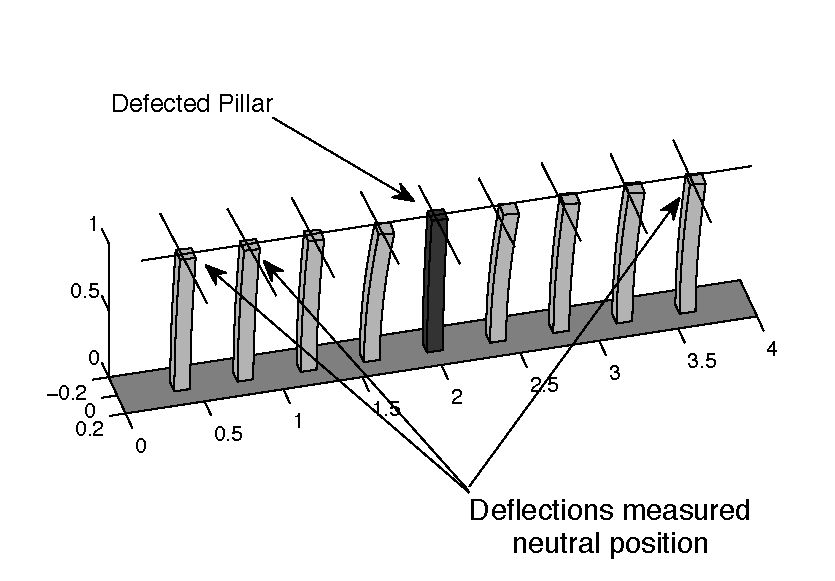
\includegraphics[width = 85mm]{../diagrams/pillarpicture.pdf}
\caption{A cartoon of one dimensional cantilever array that is able to undergo vibrations in two directions. For illustration, we have also drawn a defected pillar that is used to pin the ILM appearing from random initial condition on the center pillar. }
\label{fig:setup}
\end{center}
\end{figure}

The equations of motion for the pillars are formulated as follows. 
Let $u_k$ be the deflection of the $k$-th crystal pillar from its neutral position. A typical equation, describing the evolution of one dimensional deflection in a one-dimensional  array is given by the equation 
\begin{align} 
\ddot{u_k} = & -\alpha_1 u_k - \alpha_2 \big( (u_{k}- u_{k-1}) + (u_k-u_{k+1})\big) \nonumber   \\
 & \quad- \beta_1 u_k^3  - \beta_2 \big( (u_{k}-u_{k-1})^3+(u_{k}-u_{k+1})^3 \big)  \label{1DILMs} 
\end{align}
Here, $\alpha_1, \alpha_2, \beta_1, \beta_2$ are the constants that are determined by the  material properties of the pillars as well as the geometry. In order to describe the two-dimensional deflection of the pillars, we introduce two components of the pillar deflection as $\mathbf{u}_k=(u_{k,x}, u_{k,y})$ that are not necessarily aligned with the crystal axes. The linear components of the stress can be computed as follows. Suppose for the given deflection,  the linear part of deformation energy is given by the quadratic form $E_{2}=\frac{1}{2} \mathbf{u}_k^T Q_2 \mathbf{u}_k$. For the purpose of this paper, we choose a parameterization of the symmetric matrix $Q_2$ with three parameters $\alpha_{1,x}$, $\alpha_{1,y}$ and $\alpha_3$ as follows:
\begin{equation} 
E_2=\frac{1}{2} \sum_k  \alpha_{1,x} u_{k,x}^2+ \alpha_{1,y} u_{k,y}^2 + \alpha_3 \big(u_{k,x}-u_{k,y} \big)^2 \, .  
\label{elasticE}
\end{equation} 
For the purposes of  simplified analysis in this paper, we only consider $\alpha_{1,x}=\alpha_{1,y}=\alpha_1$ which we treat as a parameter. Then, we study the behavior of the system as a function of parameters 
$\alpha_1$ and $\alpha_3$. Note that this is somewhat different from the standard normalization, where one of the natural frequencies would be normalized to $1$. Also, it is important to notice that the eigenvalues of the Hessian of this matrix are strictly positive and distinct for $\alpha_1>0$ and $\alpha_3>0$ so there are no degeneracies or unphysical values of parameters in the system. 

The nonlinear (cubic) term in the equation leads to the fourth order term in energy, described by a fourth order tensor 
$Q_4$, \emph{i.e.}, $E_4=Q_4 \cdot \mathbf{u}_k \cdot \mathbf{u}_k\cdot \mathbf{u}_k\cdot \mathbf{u}_k$. Even when proper symmetries are included, the number of non-zero components of $Q$ lead to the exceedingly large number of parameters. It is possible to estimate some of these components analytically if the information about the orientation of crystalline axes, pillar shape and nonlinear elasticity is known. This will be done in further studies; for the purpose of this work, we shall consider a simpler particular case of the nonlinear coupling energy as 
\begin{equation} 
E_4=\frac{1}{4} \sum_k \beta_2 \Big(  u_{k,x}^4 - u_{k,y}^4 \Big)+ \beta_3 \Big( u_{k,x} - u_{k,y}  \big)^4 \, . 
\label{E4}
\end{equation} 
The total potential energy is then $E=E_2+E_4$. For symmetry reasons, in the case considered here there is no cubic term in the energy. However, note that a cubic term may appear for a general arrangement of the crystal axes and pillar facets, in the geometries breaking the reflection symmetry of the system.  The appearance and role of a cubic term in energy, leading to quadratic terms in the equations, is very interesting and will be addressed in further studies.  This will lead to the necessity of investigation of a large number of parameters, which we are not going to do here. The corresponding equations of motion for two directions are 
\begin{align} 
\ddot{u_{k,x}} = &-\alpha_{1,x} u_{k,x} - \alpha_2 \big( (u_{k,x}- u_{k-1,x}) + (u_{k,x}-u_{k+1,x})\big) \nonumber \\
& \quad- \beta_1 u_{k,x}^3  - \beta_2 \big( (u_{k,x}-u_{k-1,x})^3+(u_{k,x}-u_{k+1,x})^3 \big) \nonumber  \\
&\quad- \alpha_3 (u_{k,x}- u_{k,y}) - \beta_3 (u_{k,x} - u_{k,y})^3  \nonumber \\
&\quad \quad  -\gamma \dot{u}_{k,x} + \sigma \sin (t) 
\label{2Dx} \\
\ddot{u_{k,y}} = &-\alpha_{1,y} u_{k,y} - \alpha_2 \big( (u_{k,y}- u_{k-1,y}) + (u_{k,y}-u_{k+1,y})\big) \nonumber \\
&\quad - \beta_1 u_{k,y}^3  - \beta_2 \big( (u_{k,y}-u_{k-1,y})^3+(u_{k,y}-u_{k+1,y})^3 \big) \nonumber  \\
&\quad -\alpha_3 (u_{k,y} - u_{k,x}) - \beta_3 (u_{k,y} - u_{k,x})^3  \nonumber \\ 
&\quad \quad  -\gamma \dot{u}_{k,y} + \sigma \sin (t)
\label{2Dy} 
\end{align} 
This functional form of directional coupling allows a comprehensive study of ILM formation for two parameters, 
$\alpha_3$ and $\beta_3$. %DB: is this supposed to be a more full sentence?  ---->  The $\alpha_3$ terms denotes 
In addition, we have added the dissipation in the pillars, described by the term $\gamma \dot{\mathbf{u}}_{k}$, and the forcing term, proportional to $\sigma$. The coupling parameters $\alpha_3$ and $\beta_3$ can be estimated numerically, but their precise value for a given experiment is generally unknown. Thus, they must be treated as parameters in the problem.    
\section{Results} 
Here, we present the results for spontaneous formation of ILMs in the system.  The values of other parameters are presented in the table below. For completeness, we present the values of the other parameters used in simulations below. 
While the typical value of $\alpha_1$ are around 1, we have chosen to scan a large set of values in order to accommodate both cases when there is large discrepancy in natural frequencies in two directions, and, alternatively, when the 
natural frequencies of vibration are very close to each other.  
\begin{center}
\begin{tabular}{|c|c|}
\hline Parameter & Value \\
\hline
 $\alpha_1$ & 0.0001 \ldots 1 \\
 \hline 
 $\alpha_3$ & 0.0001 \ldots 1 \\
 \hline 
 $\beta_1$ & 0.01  \\
 \hline 
 $\beta_2$ & 0.0001 \\
 \hline 
 $\beta_3$ & 0, 0.001 \\
\hline
$\gamma$ & 0.001 \\
\hline 
$\sigma$ & 0.01 \\
\hline 
\end{tabular}
\end{center}

The results of our simulations are presented on Fig.~\ref{fig:phase1} and Fig.~\ref{fig:phase2}. We plot the ILM detectability, \emph{i.e.}, the energy concentrated in an ILM divided by the average energy of a pillar, which is non-zero due to the competition between the forcing and dissipation.  Each point on this plot is the result of simulation until $t=300$, with the amplitude of ILM computed from the last half of the time interval. The horizontal and vertical axes are $\alpha_3$ and $\alpha_1$, respectively. Red areas represent high values of detectability, and blue represent the low values. As we see, there are areas of parameter where ILM appearance is very robust; however, these areas are relatively small.  There is a highly intricate pattern describing high detectability of ILMs, and it is more typical to observe the energy concentration in ILM to be rather small, as is evident from our results. Thus, the preliminary work presented here warrants more detailed studies of ILM formation and detectability, and the necessity of improved design of nanopillar arrays for nanotechnology applications. 


\begin{figure}[t]
\begin{center}
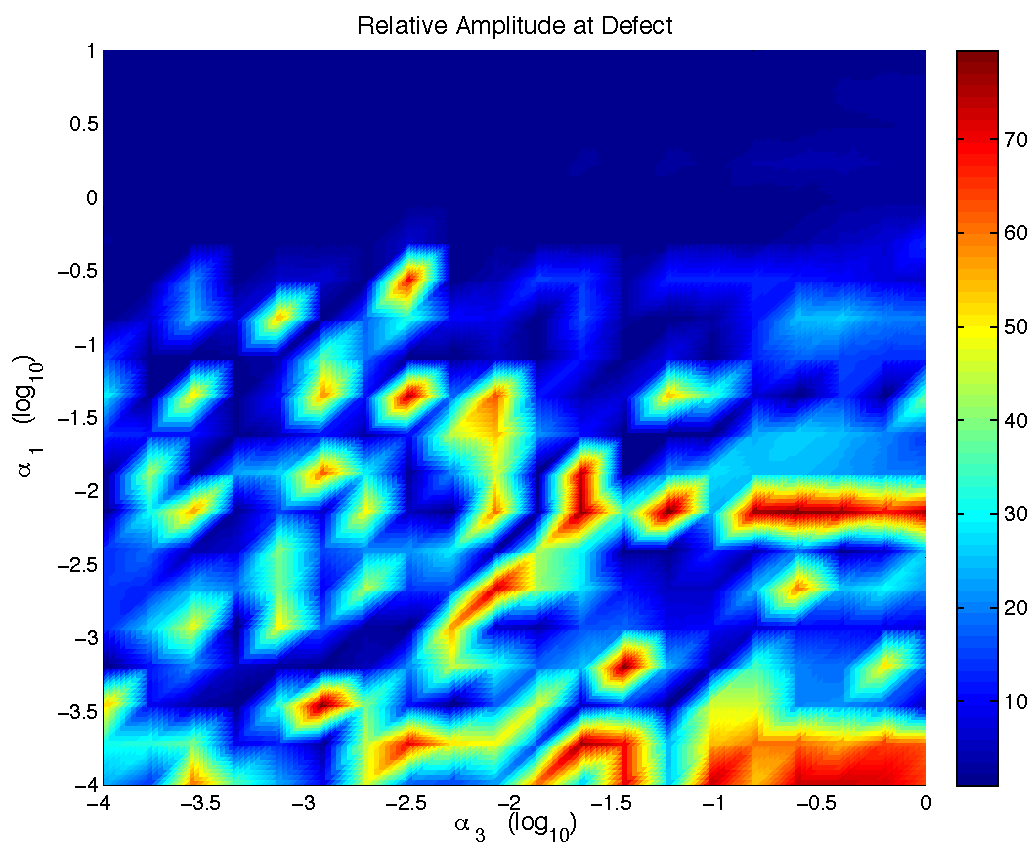
\includegraphics[width = 83mm]{../diagrams/alpha13beta0.pdf}
\caption{Phase diagram for ILM presence in 9-pillar crystal array.  Coupling parameters $\alpha_1$ and $\alpha_3$ are examined for  $\beta_3=0$. Red denotes strong ILM formation whereas blue indicates practically no spontaneously forming ILMs present in the system. In order to scan large areas of parameters we use logarithmic scale for $\alpha_1$ and $\alpha_3$. }
\label{fig:phase1}
\end{center}
\end{figure}

\begin{figure}[t]
\begin{center}
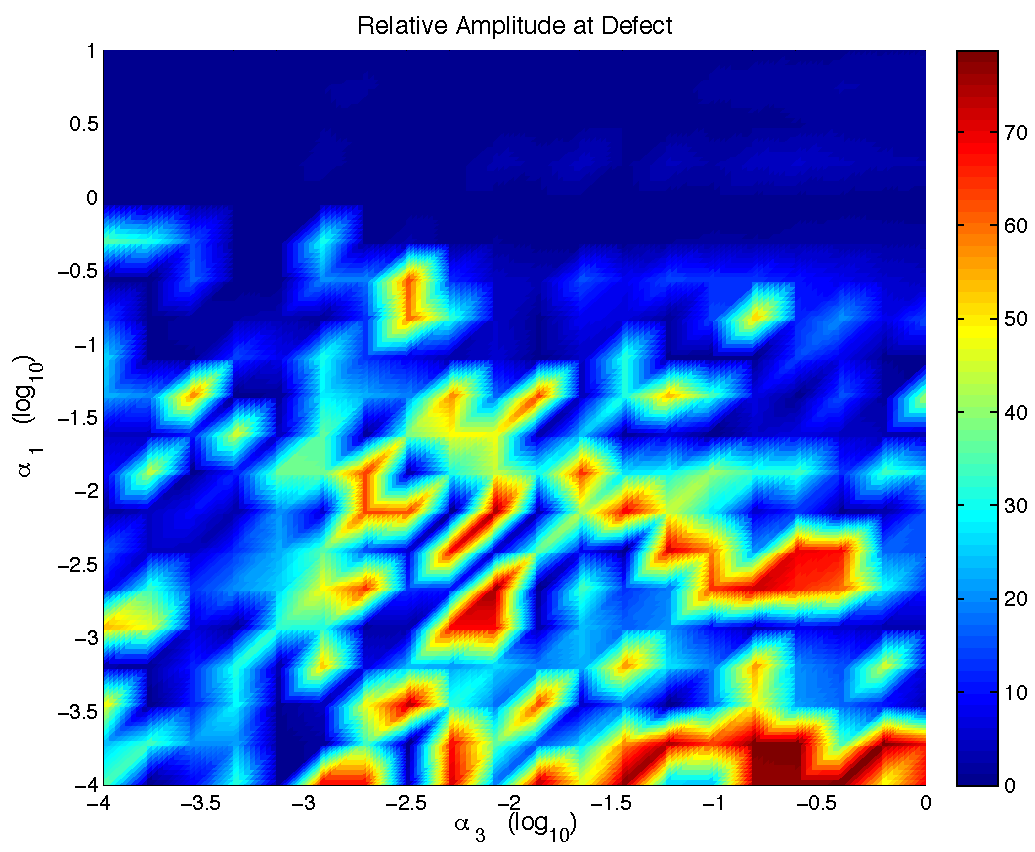
\includegraphics[width = 83mm]{../diagrams/alpha13beta3small.pdf}
\caption{Same phase diagram as in Figure~\ref{fig:phase1} but computed for $\beta_3=0.001$}
\label{fig:phase2}
\end{center}
\end{figure}



\section{History and Motivation}
\section{Single Molecule Detection through Intrinsic Localized Modes}
	
\section{Using \bertini to Find ILM}
	








%%%%%%%%%%%%%%%%%%%%%%%%%%%%%%%%%%%%
%
%
%               ROBOTIC WORKSPACES CHAPTER
%
%
%%%%%%%%%%%%%%%%%%%%%%%%%%%%%%%%%






\chapter{Cooperative Robotic Workspaces}


Fault-tolerance and robustness play important roles in the design of autonomous systems, including robotic arms.   In this paper, we consider  autonomously operated robotic systems that are deployed into a hazardous or remote location, such that the repair on a failed joint is impractical or impossible.  If the system has to operate for an extended period of time, we want the system to operate to the best of its 
remaining physical capability after a joint failure. 

Suppose such a system possesses several robotic  arms for various tasks.  While no robot can be completely fail-proof, under normal operating conditions the probability of several joints failing simultaneously is low.  Thus, we are considering only one joint failure at a time.   We also assume the robots cannot change their position with respect to one another.  Then, should one joint in one arm fail,  the presence of a second arm may open the way to preserve some of the workspace of the failed arm.  In particular, if the second arm can grasp the first, perhaps some of the lost workspace of the first arm can be restored.  


Immediately, two questions arise: \emph{a)} What is the best placement of the robots in relation to each other?   \emph{b)}  Is there a best place for the second arm to grasp the first? 
We should mention here that the answer to both questions clearly depends on the measure of the post-failure workspace, which is problem dependent. In this paper, we use the Euclidean measure in $\mathbb{R}^3$, corresponding to the embedding of the workspace, to quantify the size of the workspace.  In general, the user suitably introduces a measure corresponding to the robot's embedding space including position and orientation, and problem type; other measures (for example, closeness to a target) will change the details of the optimization procedure, but the basic structure of the solution process should remain unchanged.  Our focus in this paper is 
to find the optimal separation and grasp point for one robot to grasp another in the event of a free-swinging joint failure, so as to maximize the area of the post-failure workspace. To solve this problem, we use the method of homotopy continuation.  In particular, the inverse kinematics problem can be cast as a polynomial system, and homotopy continuation provides a means for efficiently producing numerical approximations of \emph{all} isolated complex and real-valued solutions of the polynomial system.  

%We recognize that, for this particular case, the problem could be solved in almost closed form.  However, this traditional approach fails to generalize when additional degrees of freedom are present, \emph{e.g.} higher dimensions or more links, whereas our approach is directly transferrable to higher dimensions.


Consideration of fault-tolerance is essential in dangerous locations, and has been studied extensively.  Difficulties arising from considerations of reliability and safety were pointed out in the review  \cite{DFL02}.  The detection and isolation of faults, in various components of a robot, such as sensors, controllers, and actuators, as well as collision with environmental elements, was treated in \cite{ASKJ07,JS07,DF09,BCFP08}.  Anticipation of failures has also been explored considerably;  decomposing a task into primary and secondary goals is one method of dealing with these problems.  Prioritization of tasks subject to other constraints (\emph{e.g.},environmental) was treated in \cite{CMY03,LM97}, while paper \cite{EM98} studied the anticipation of free-swinging joint failures.   The failure-tolerant region of workspace was defined in \cite{GMB99}, which also gave a method for computing a fail-tolerance measure which allows a robot to operate within this fail-tolerant region  in real time.  Other measures of fail-tolerance include analysis of the singular values of the Jacobian matrix for a robot \cite{Mac90} and a `manipulability index' as defined in \cite{RM96}.
Robots can be designed and operated with fail-tolerance in mind, such as dual actuators at joints \cite{HN07}, kinematic redundancy \cite{MON99,HN07,WHC93,YMC06,PK96}, and reconfigurability \cite{AgPa2009}.  Determining the reliability of a robot via fault-tree analysis appeared in \cite{CW01}, which allows to quantify weaknesses in design.  

The key feature of this manuscript is the application of methods of algebraic geometry to the description of fault tolerance of two cooperating robots.  
These techniques are guaranteed to give all isolated solutions to algebraic equations describing the positions of robotic arms, and thus robustly find solutions in arbitrarily complex settings, such as multiple roots and joint values in isolated regions of joint-space. 
Thus, these techniques are capable of \emph{autonomously} completing the workspace analysis, which can be useful in robots operating with high degree of independence, with little or no communication with the operator. The trade-off for the completeness of analysis is the computational complexity as compared to \emph{e.g.} the Jacobian control methods, as we show below.  If extra information about the workspace, such as the exact number of isolated domains and multiplicity of solutions is available, then traditional methods will be advantageous computationally. If no such \emph{a priori}  information is available, the methods we describe here should provide precise information about the isolated domains and solution multiplicity which, if desired, can be further refined by Jacobian control methods. 


Methods of algebraic geometry have been applied in the kinematic description of robots as well,  see for example \cite{SW05,SVW04,WM93,WMS92,WaHaSo11}. However, analysis of the cooperation of multiple arms via the tools of numerical algebraic geometry has never been explored.  
In the next section, we provide a formal statement of the general problem we are considering.  Background regarding the numerical solution of polynomial systems may be found in Section \ref{sec:bertini}.  Details about our method are described in Section \ref{sec:workspacecomputation}, while Sections \ref{sec:twojoint} and \ref{sec:threejoint} respectively contain two and three dimensional examples.



\section{Formal Problem Statement} \label{sec:probstatement}

Given two articulated arms, we seek to optimize the placement of grasping sockets to maximize the post-failure workspace (we assume a socket attachment mechanism of the first arm to the second as considered in  \cite{AgPa2009}). That is, if one robot has a free swinging joint failure \cite{EnMa2000,EnMa2001}, we would like to ensure that when the functional robot joins at the socket, the resulting cooperative workspace is as large as possible. 


Each robot has its own independent workspace, (let us call them $W_1, W_2$), so  when the two robots are placed near enough to each other, there is an intersection workspace $W_\cap$ = $W_1 \cap W_2$.  In a grasping configuration, there is a post-failure workspace $W_f$, which contains all remaining workspace, if robot 2 attaches to the socket location on robot 1.  It is clear that $|W_\cap|$ depends on the separation between the robots, as well as their orientation, as does $|W_f|$.  Note that the intersection workspace does not depend on the grasping point, as it reflects the workspace prior to failure for each robot. In  both pre- and post-failure workspaces, we take into account joint limits, which are an important consideration for practical applications. Indeed, 
robots typically have limited range of movement for each joint, which reduces the size of all workspaces.  These limits introduce a dependence on the relative rotations of the robots to each other, to the measures of the various workspaces.

An optimal configuration of two cooperating robots would include: the separation between the cooperating arms, the relative orientation of the bases, and the location of the grasping point for each link.  In order to give quantifications about the post-failure workspace size and consequently find such an optimal configuration, we introduce an objective function, which we seek to maximize.  There are many possible objective functions one can imagine, and the right choice depends on the application. In this paper, our
objective function to be maximized is a weighted sum of $|W_f|$, $|W_1|$, and $|W_\cap|$:
\begin{equation}
\Omega = (1 - \lambda) \cdot |W_f| + \lambda(|W_1|  - |W_\cap|).
\label{Omegadef}
\end{equation} 

We have chosen (\ref{Omegadef}) for an example objective function in order to balance between the benefit of having a second robot, and the maximization of the post-failure workspace.  A configuration which imparts entirely distinct workspaces would maximize the term $\lambda(|W_1|  - |W_\cap|)$, but $W_f$ would be an empty set.  Contrarily, we might find a configuration which results in full restoration of workspace $W_f$ upon entering grasping stance, but which makes the pre-failure workspaces overlap greatly, so $ \lambda(|W_1|  - |W_\cap|)$ would be small.  We would prefer to balance between pre- and post-failure benefits of having two robots, and (\ref{Omegadef}) is one way of doing this.

\section{Homotopy Continuation} \label{sec:bertini}

We recast the inverse kinematic problems for computation of (\ref{Omegadef}) in the form of polynomial systems, and use the  methods of numerical algebraic 
geometry, particularly homotopy continuation, to find the solutions of these polynomial systems.  Given a set of polynomials $f_1,\ldots,f_N$ in $N$ variables for which we 
seek the solutions, homotopy methods begin by choosing and solving some other (related) polynomial system $g_1,\ldots,g_N$ for which the solutions are easily found, e.g., polynomials such as $x^6-1$.  By varying the coefficients of $\bar{g}$ to those of $\bar{f}$, mathematical theory guarantees that, with probability one, the solutions will 
vary continuously, thus forming {\em solutions curves} or {\em paths} from the solutions of $\bar{g}$ to those of $\bar{f}$.  These solution curves may then be tracked numerically 
with standard predictor/corrector methods, such as a combination of RK45 and Newton's method.   Further details may be found in~\cite{AG90,SW05}.

There is a setting in which homotopy methods are particularly effective and of which we make use in this paper.  If instead of solving one polynomial system $\bar{f}$  we wish to solve a large number of polynomial systems that differ only in their coefficients (i.e., we wish to solve $\bar{f}(\bar{p})$, where $\bar{p}$ is some set of parameters), there is an especially efficient homotopy method known as a {\em parameter homotopy}.  The key of the method is to have a simple system $\bar{g}$ for $\bar{p}=\bar{p}^*$, and find a path in the parameter space leading to the system of interest as $\bar{p}=\bar{p}_0$. When constructing a starting system $\bar{g}$, it is possible that there will be many more solutions of $\bar{g}$ than $\bar{f}$.  As a result, it may occur that hundreds of thousands of  solution curves are tracked in order to find only a few solutions.  However, in the special case of a parameter homotopy, we first solve $\bar{f}(\bar{p})$ at a single instance of  $\bar{p}^*$ (typically chosen as random complex numbers, for theoretical reasons).  This stage may involve a number of wasted paths.  All other instances of $\bar{f}(\bar{p})$ may then be solved by simply following the handful of finite solutions from $\bar{p}^*$ to any other choice of $\bar{p}_0$.  For example, for an initial, random complex parameter choice, we may need to follow thousands of paths to find the six solutions of interest.  Then, for all other points in the parameter space, it suffices to follow just six paths.  Again, there is much theory and detail underlying these methods, most of which may be found in~\cite{SW05}.  During the process of homotopy continuation, a certain number of paths will fail as they near a singularity in parameter space.  In the context of robotic workspaces, these failed paths indicate proximity to workspace boundary or kinematic singularity.  Right now, we are not using this information, and simply ignore failed paths;  however, that property could ultimately be used for more accurate and efficient prediction of, for example, workspace boundaries.


For this paper, it is enough to accept homotopy continuation as a numerical method that will provide approximations to all isolated solutions of a polynomial system.  Several software packages are available for these sorts of computations.  We use a freely-available software package named \emph{Bertini}~\cite{Bertini}, which has been under development for the past decade by the second author, J.~Hauenstein, A.~Sommese, and C.~Wampler.   The repeated calls to \bertini~were parallellized for efficiency using the method described in \cite{BrBaNi11}.







\section{Workspace Computation} \label{sec:workspacecomputation}

%\subsection{$W_i$ Computation} \label{sec:w_icomputation}


We compute the initial pre-failure workspaces for each robot via a random sampling method. We sample a subset of  the space which embeds the workspace, that is guaranteed to contain the workspace, using a uniform pseudo-random distribution with the built-in MATLAB random number generator, solving the inverse kinematics problem at each of these sample points, as follows.

The equations for the inverse kinematics problem are first solved via a standard homotopy run at 
$\bar{p}^*$, a random point in complex parameter space. All subsequent runs at parameter points in the workspace are treated as parameter homotopies, and all such runs begin at $\bar{p}=\bar{p}^*$. 
Because \emph{Bertini} will find all complex solutions to a polynomial system, the samples that result in real inverse kinematic solutions are inside the workspace, while samples that gave only complex solutions are outside the workspace.  If we have $r_i$ samplings, and $r_f$ of these have real solutions, we can estimate the (Euclidian) measure of the workspace as the product of the volume of the sampled box, and the ratio $r_i/r_f$.  


We shall note that the inverse kinematics equations for a robot with rotary joints are trigonometric in nature.   In order to use homotopy continuation, we  write the trigonometric equations in a polynomial form by treating each sine and cosine pair as a separate variable, mapping $\cos(\theta_i) = c_i$ and $\sin(\theta_i) = s_i$.  Then, trigonometric variables can be recast into algebraic conditions using $c_i^2+s_i^2=1$. 


%Taking $L = 1$, we write the inverse kinematics equations as:
%\begin{align}
%0 = \left\{ \begin{array}{r} c_1c_2 - s_1s_2 + c_1 - P_x  \\
% s_1c_2 + c_1s_2 + s_1 - P_y \end{array}  \right.  .\label{eqn:inv1} 
%\end{align}
%These equations are augmented by trigonometric identities,
%\begin{align}
%c_i^2 + s_i^2 - 1 &= 0 ,\quad i = 1,2.\label{eqn:inv2}
%\end{align}
%Four total equations (\ref{eqn:inv1},\ref{eqn:inv2}), in four unknowns, constitute the polynomial system we will solve using the homotopy continuation solver \emph{Bertini}.  We treat $P$ as a parameter.  

%The solve is performed in two steps: first, an initial solve for random complex values of $\bar{p}^*$; second, a solve for each of the $r_i$ samples, with $\bar{p}$ as the sample itself.  The advantage of using a parameter homotopy in this case is a great reduction of computation time.  For example, using a two-link rotary robot, the initial solve tracks eight paths to find two complex solutions, and the second solve tracks two paths to two solutions, giving a speedup of 4.  In other words, without using parameter homotopies, each solve would require the tracking of eight paths rather than two.

For the case of $N\geq3$ joints working in $3$ dimensions without orientation, there are 6 inverse kinematic equations in $2N$ variables when computing $W_i$.  As long as the number of joints equals the number of degrees of freedom in the ambient workspace, \emph{Bertini} will find all solutions, and we will be able to measure $|W_i|$.  For kinematically redundant robots, $W_i$ is a set of higher $2N-6$ dimensional manifolds, which could be described by defining a mesh of the same dimensionality as coordinates on the joints.  Our method readily applies to that higher dimensional problem as well.  However, the issues we are facing are related to the curse of dimensionality, and hence in the computation of the data as a whole, not in the solution finding at a particular point in space, which is fast.  For example, with $N=5$ joints, and a 3 dimension workspace, each point in the workspace is a two dimensional manifold in joint space.  To cut down the manifold to be 0-dimensional for solving via \bertini, we could sample each of the two redundant joints' values.  Combinatorial issues arise as well, if we wanted to solve each spatial sample for each possible combination of redundant joints.  The work load increases dramatically with the growth of dimensionality for both the robot and ambient workspace.  Another problem is whether to use random spatial sampling or a mesh, and how to optimize the number of samples.  The optimal sampling will depend on the geometry of the manifolds, and has to be studied in more detail elsewhere.  

%In any case, the problems we are facing regarding extending this method to higher dimensions do not come from the method itself, but from sampling and data analysis issues.  Thus, while our method is general and rather powerful, more work will be needed to apply it to complex configurations. 

%








%\subsection{$W_\cap$ Computation} \label{sec:w_capcomputation}

A similar computation is performed to find an estimate of $|W_\cap|$. Because we know that $W_\cap \subset W_2$, we simply solve the inverse kinematics of robot 1 at the $r_f$ points that gave real solutions for $W_2$. Suppose that of $r_i$ initial samples, $r_f$ gave real solutions for $W_2$, and $r_k$ correspond to a real solution belonging to 
 $W_1$, then we can estimate the intersection work space to have measure 
\[
|W_\cap| \approx \frac{r_f}{r_k} .
\]






%\subsection{$W_f$ Computation}  \label{sec:w_fcomputation}

The final component for calculating the objective function is to estimate the post-failure space $|W_f|$.  Note that there is an associated space for each link of the failed robot, as we could potentially join a specially placed socket on each link.  
%
We know that $W_f \subset W_1$, so as for $W_\cap$, we need only consider the $r_f$ points we computed in $W_1$.  The major difference between the computation of $W_{1,2}$ and $W_f$ is the number of equations which is twice as high for the $W_f$ computation. 
%


%The maximum resulting workspace with respect to varying $a$ for a given $\delta$ determines the optimal  placement of, for example, a grasping location on robot one, to ensure the largest restored workspace in the event of a free-swinging failure of the second joint of robot one.










\section{2D case: Two link planar robots} \label{sec:twojoint}


\begin{figure}
\begin{center}
	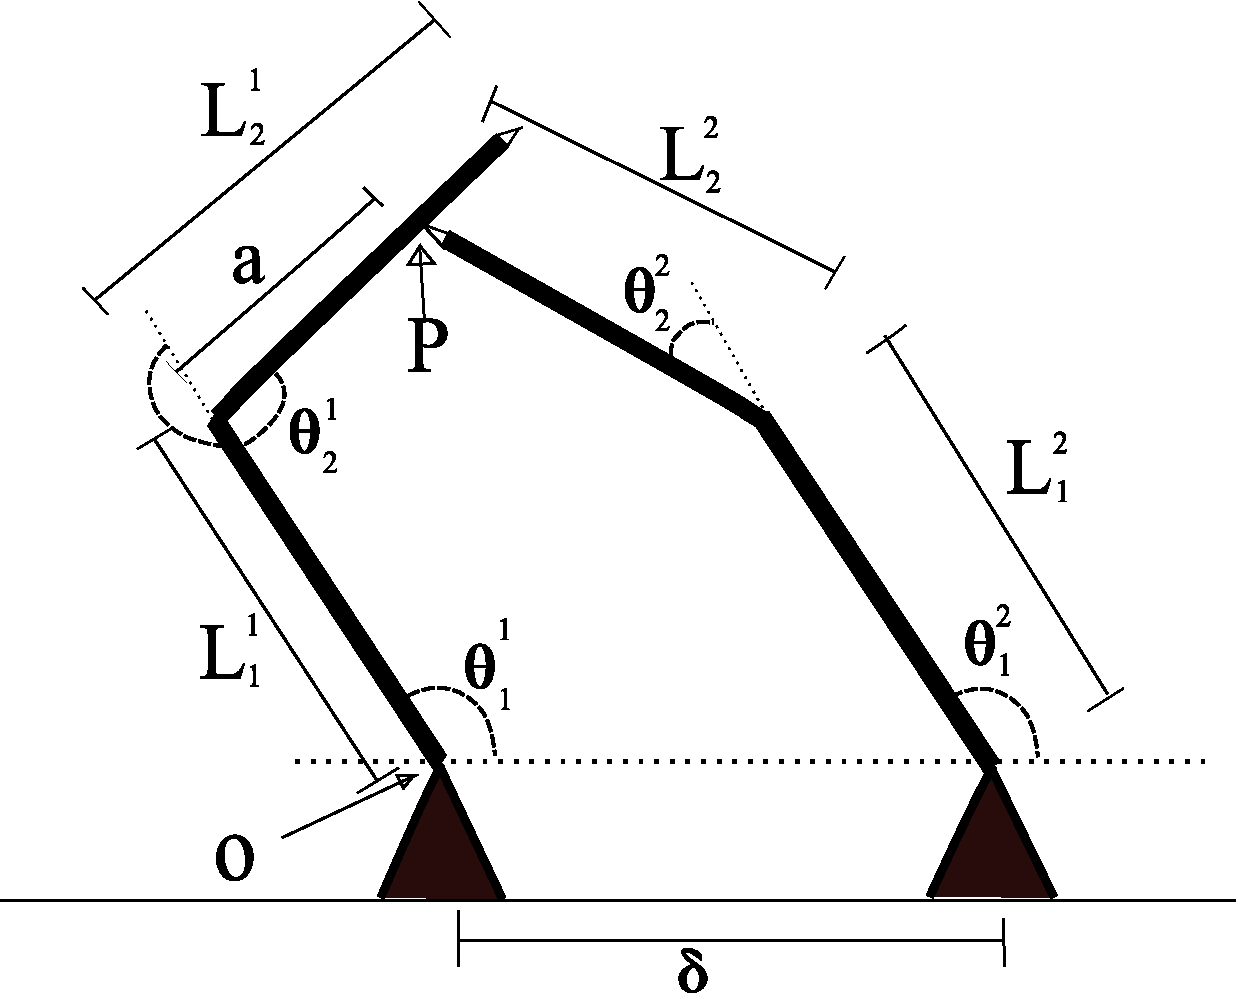
\includegraphics[width=3.25in]{../diagrams/RRtimestwo.pdf}
	\caption{\small{Two robots touching at point P. This is a simplified 2D model of a more general scenario. In this paper we will not consider the final arm orientation.}}
	\label{fig:TwoRobotsTouchingAtPointP2}
	\end{center}
\end{figure}

We start with the illustration of the method for 
a two dimensional example that is  shown in Figure~\ref{fig:TwoRobotsTouchingAtPointP2}. We have chosen this example because almost all inverse kinematic equations can be explicitly inverted, so this problem represents a good test case for our method.  We first considered this in \cite{BBPM10}.  The more challenging three-dimensional problem is considered later in Section~\ref{sec:threejoint}. 

Let the separation distance be $\delta$ and let this translation between  coplanar bases be entirely along the $x$-axis; we will sort out-of-limit solutions in a post-processing procedure.  We consider $0<\delta<4$, the largest value of $\delta$ corresponding to the robots barely reaching each other.  The normalized distance to the  grabbing point measured from the failed joint is denoted by $a$, with $0<a<1$.  Also let the point at which a socket is attached to the left robot, hereafter robot 1, be point $P$, with the origin at the base of robot 1.  Finally, let the fully functional machine be known as robot 2.

There is some probability that each joint could fail, so it is important to take into consideration the placement of a socket on each link.  We use the Denavit-Hartenberg convention to describe the configurations of the two robots.  Then we can describe the contact point $P$ in terms of the DH parameters for robot 1, as  $P$ is some distance $a$ from the origin of the previous frame.   A spatial sample $Q$ can then be said to be in the post-failure workspace of robot 1 for a parameter pair $(\delta,a)$, if there exists a set of joint angles such that end effector of robot 1 is at $Q$, and the end effector of robot 2 is at $P$.


%In our case, the post-failure workspace $W_{f}$ is a subset $\R^n$; if we are considering orientation at each point in this space, we must consider the direct product of $SO(n)$, the set of rotations in two-space, and $\R^n$.  


It seems that one obvious way to maximize $| W_f |$ is to set $\delta =0$ so the two robots have exactly the same base point,  and make the two robots identical. However, this is an impractical situation. First of all, there may be much greater benefit to having greater pre-failure workspaces by placing the robots further apart, and second, depending on the robot geometry, it could be awkward or impossible to place two identical robots operating from the same base point.


To demonstrate the method, we show results for a uniform random sampling of $n = 10^3$ points for contour plots, and $n= 10^5$ for $W_f$ plots.  The robots are identical, both having two joints, all normalized to length one.
To start with, we uniformly sample a two dimensional rectangle which surely contains the workspace of robot two.  A reasonable set of bounds are $\bar{p} = (x,\,y) \in [-2,2]\times[-2,2]$.  To see the typical computation workload involved in the computation of $W_i$, we sampled initially $r_i=10000$ times, and only $r_f=7836$ of these points had at least one real solution, the estimated size of the workspace would be $|W_1| =4^2 \times 7836/10000 \approx 12.5$.  However, it is often more convenient to work with normalized measures; we will hereafter normalize with respect to the measure of the initial sample.  Therefore the normalized measure of an initial workspace is simply $r_i/r_f$, and of this example is $7836/10000 \approx 0.783$.


Let $i \in \{1, 2, 3, 4\}$, so that we have a sine-cosine pair for each of the two joints in the two robots. 
We want to place the robots in such a way that robot 2 touches robot 1 at point $P$. 
%Then, for a given value of parameter $a$, we have a secondary DH table for robot 1:

\begin{table}
\begin{center}
\caption{Denavit-Hartenberg Parameters for two-link planar robot.}
\label{tab:2ddh}
\begin{tabular}{| c | c | c | c | c | c |}
\hline
$\theta_i$			&	$\alpha_i$			&	$a_i$	&	$d_i$		&  $\theta_{i,min}$	&	$\theta_{i,max}$\\ \hline
$\theta_1$ 		&	0					& 	1		&	0			& $-120^\circ$	& $120^\circ$ \\
$\theta_2$ 		&	0					& 	1		&	0			& $-45^\circ$	& $45^\circ$\\
\hline
\end{tabular}
\end{center}
\end{table}

%\[
%DH =  \begin{bmatrix}
%\theta_1 		&	0				& 	1		&	0\\
%\theta_2 		&	0				& 	a		&	0 
%\end{bmatrix}.
%\]
%
Here, we define $c_i$ and $s_i$ to be the cosine and sine, respectively, with $i=1,2$ corresponding to the first (failed) robot and $i=3,4$ corresponding to the second (assisting) 
robot. 
In this notation, our equations for this step are,
%
\begin{align}
0 = \left\{ \begin{array}{l}
c_1c_2 - s_1s_2 + c_1 - x  \\
s_1c_2 + c_1s_2 + s_1 - y \\
ac_1c_2 - as_1s_2 + c_1 - (c_3c_4 - s_3s_4 + c_3+ \delta) \\
as_1c_2 + ac_1s_2 + s_1 - (s_3c_4 + c_3s_4 + s_3)\\
s_i^2 + c_i^2 - 1  \end{array}
 \label{2Deqs} 
\right.
\end{align}
We consider $\delta$, $a$, $x$, $y$ to be parameters for \emph{Bertini}.  We again solve these systems in two steps.  Using the two-step procedure described above, the initial random solve involves 16 paths, and the subsequent parameter solves involve only 4 paths. 


%
%\begin{figure}
%\begin{center}
%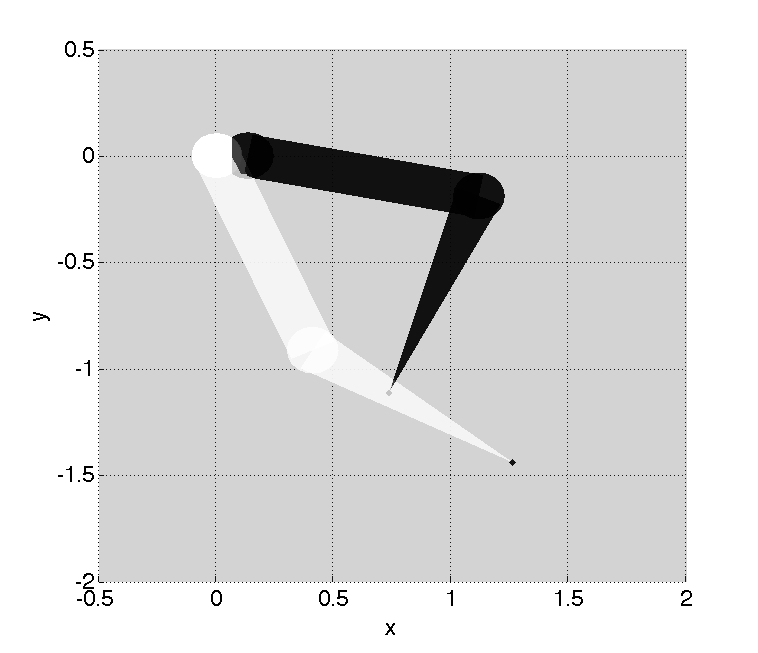
\includegraphics[scale=0.38]{../diagrams/demograsp_0133_0381.png}
%\caption{{\small Demonstration of grasping configuration.  In this randomly chosen example, $a=0.381$ for $\delta = 0.133$.}  }
%\label{fig:demograsp}
%\end{center}
%\end{figure}
  For each point in the sampling, we determine whether it lies in the desired space, by the above described method of homotopy continuation, using the inverse kinematic equations for the Denavit-Hartenberg parameters.  
  
  Because \emph{Bertini} solves over the complex numbers for each variable, we find solutions for each point, regardless of whether it lies inside the workspace.  However, the points that have solutions for which all variables are real-valued (numerically real-valued, calling zero any imaginary part less than $10^{-4}$), are those lying within the  workspace.    
The first step in the computation is to compute the workspace for both robots, as described in Sec.~\ref{sec:workspacecomputation}.  Because the robots are identical in this example, there is only one workspace computation.
The second step in computation is the intersection of the two workspaces, for a specified set of $\delta$ values.
Finally, for each pair of values ($\delta,a$) for which we estimate the post-failure grasping workspace, we solve a set of equations (\ref{2Deqs}).  For this example, we computed $W_f$ for the set of $\delta$ and $a$, with $|W_f|$ normalized with respect to $|W_1|$.





%% \begin{figure*}[t]
%% \begin{center}
%% 	\subfigure[$\delta = 1.067$.]{
%% 		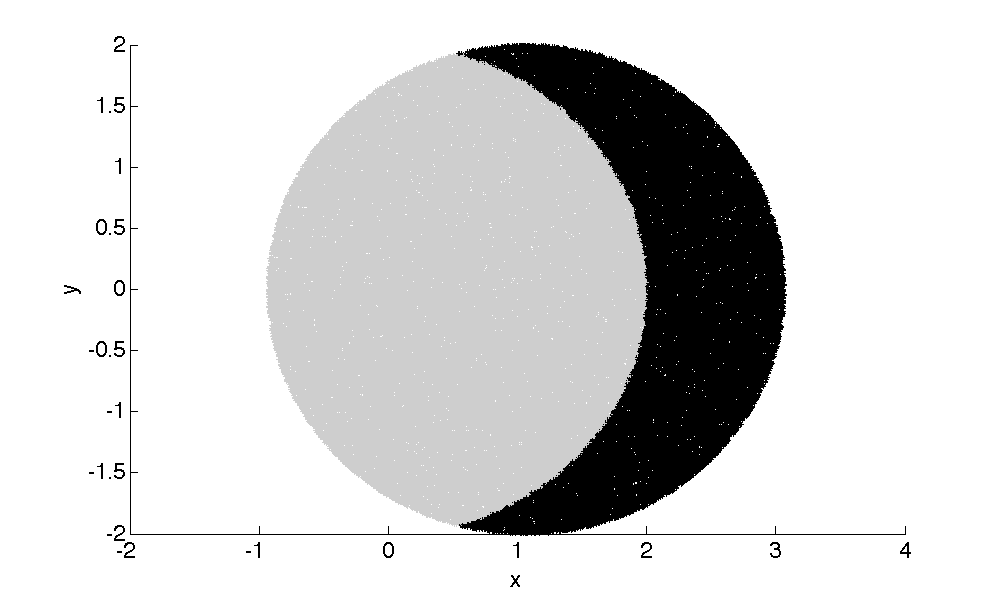
\includegraphics[width=3in]{../diagrams/isect-1067dot.png}
%% 		\label{fig:isect_1067}}
%% 	\subfigure[$\delta = 2.933$.]{
%% 		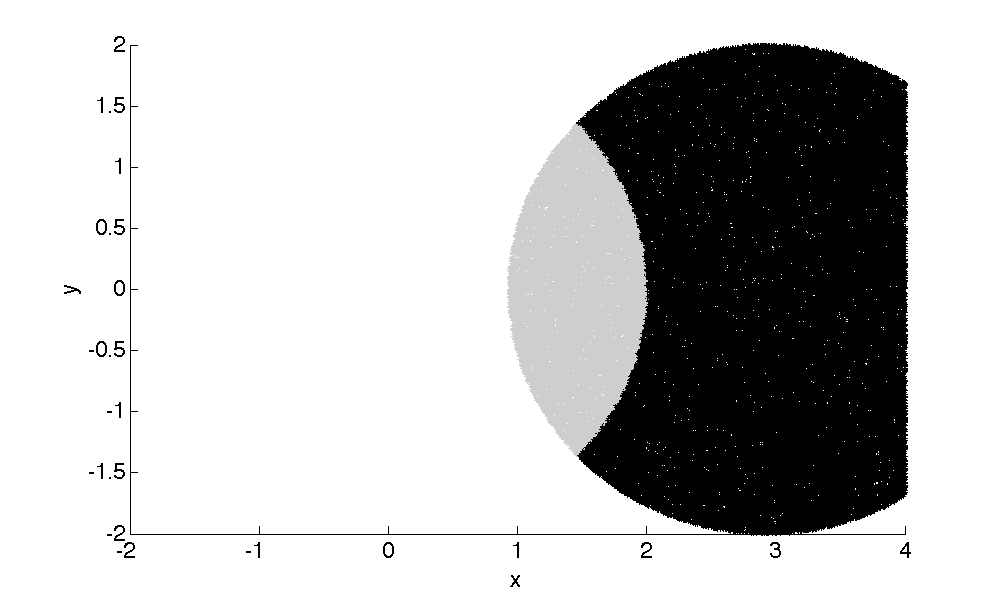
\includegraphics[width=3in]{../diagrams/isect-2933dot.png}
%% 		\label{fig:isect_2933}}		
%% 	\caption{{\small Example $W_\cap$, for $n = 150000$ points.  Black area is not in the intersection workspace, while gray lies within.  Not surprisingly for these two robots, the computed spaces are merely intersections of circles.  More complicated shapes are expected for different robot configurations, and for robots working in $\R^3$.}}
%% \end{center}
%% \end{figure*}

%% \begin{table}[t]
%% \begin{center}
%% \begin{tabular}{|c|c|}
%% \hline 
%% $\delta$ &  \\ \hline
%% 0      & 1 \\
%% 1.067  & 0.663 \\
%% 2.050  & 0.378 \\ 
%% 2.933  & 0.159 \\ 
%% $>4$   & 0 \\ \hline
%% \end{tabular}
%% \end{center}
%% \caption{{\small Normalized intersection workspace sizes, computed from a sampling of $n = 150000$ points.}}
%% \label{tab:w_cap}
%% \end{table}%

\begin{table}[t]
\begin{center}
\caption{{\small Estimates on the normalized size of post-failure workspaces, with robot 2 grasping robot 1.}}
\begin{tabular}{|c|c|c|c|}
\hline 
$\delta$ & $a$ & $|W_\cap| / |W_1|$ & $|W_f|/|W_1|$ \\ \hline
0     & $\forall a \in [0 , \, 1]$ & 1 & 1 \\ \hline
 			& 0.1 & 			& 0.98\\
1 		& 0.5 & 0.68 	& 0.86\\
 			& 0.9 & 			& 0.72\\ \hline
 			& 0.1 & 			& 0.64\\
2 		& 0.5 & 0.39 	& 0.54\\
 			& 0.9 & 			& 0.42\\ \hline
 			& 0.1 & 			& 0.07\\
3 		& 0.5 & 0.14	& 0.14\\
 			& 0.9 & 			& 0.15\\ \hline
$>4$  & $\forall a \in [0 , \, 1]$ & 0  & 0 \\ \hline
\end{tabular}
\end{center}
\label{tab:w_f}
\end{table}




\begin{figure}
\begin{center}
	\subfigure{%[$(\delta,\,a) = (1,\,0.5)$.]
		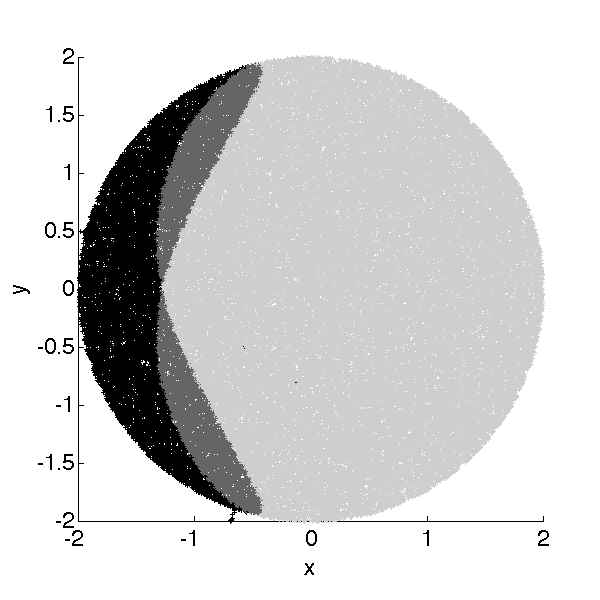
\includegraphics[width=1.03in]{../diagrams/grasp_delta1_a05.png}
		\label{fig:grasp_1_0.5}	}	
	\subfigure{%[$(\delta,\,a) = (2,\,0.5)$.]
		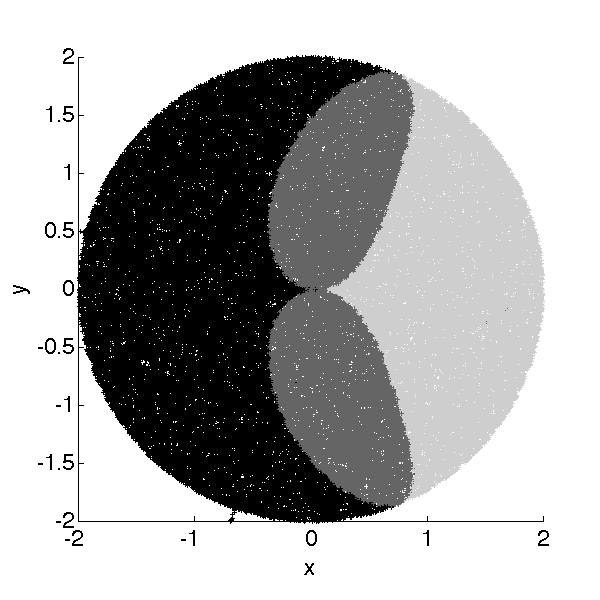
\includegraphics[width=1.03in]{../diagrams/grasp_delta2_a05.png}
		\label{fig:grasp_2_0.5}}		
	\subfigure{%[$(\delta,\,a) = (3,\,0.5)$.]
		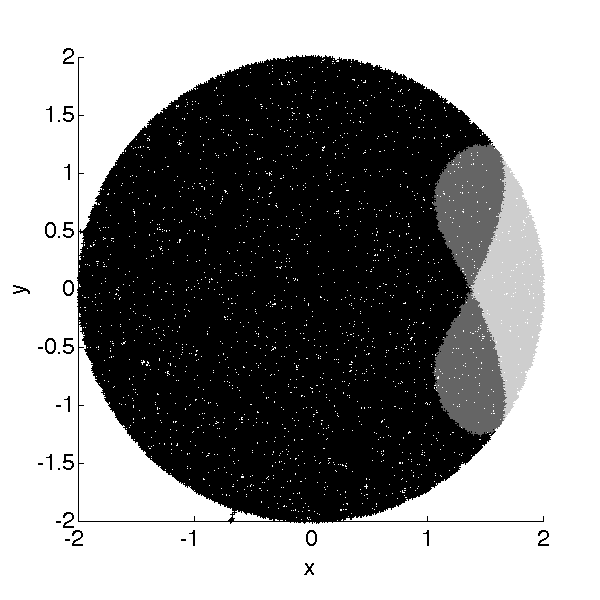
\includegraphics[width=1.03in]{../diagrams/grasp_delta3_a05.png}
		\label{fig:grasp_3_0.5}}	
	\caption{ 
	 Example of $W_f$ for $a=0.5$ and $\delta=1,2,3$. Black points are not reachable in the post-failure space.  Dark gray areas are reachable in two configurations, as one for robot 1, and two for robot 2.  Light gray areas are reachable in four configurations (two per robot).
	}
	\label{fig:spaceshape}
\end{center}
\end{figure}


Using a sampling of $n = 1000$ points, we computed both $|W_\cap|$ and $|W_f|$. The size of the intersection workspace is  monotonically decreasing as we increase the separation distance. This makes geometric sense because $W_\cap$ is merely the intersection of two circles.  See Figure~\ref{fig:w_cap} and column three of Table~\ref{tab:w_f}.

\begin{figure}[t]
\begin{center}
\subfigure[$|W_\cap|(\delta)$.]{
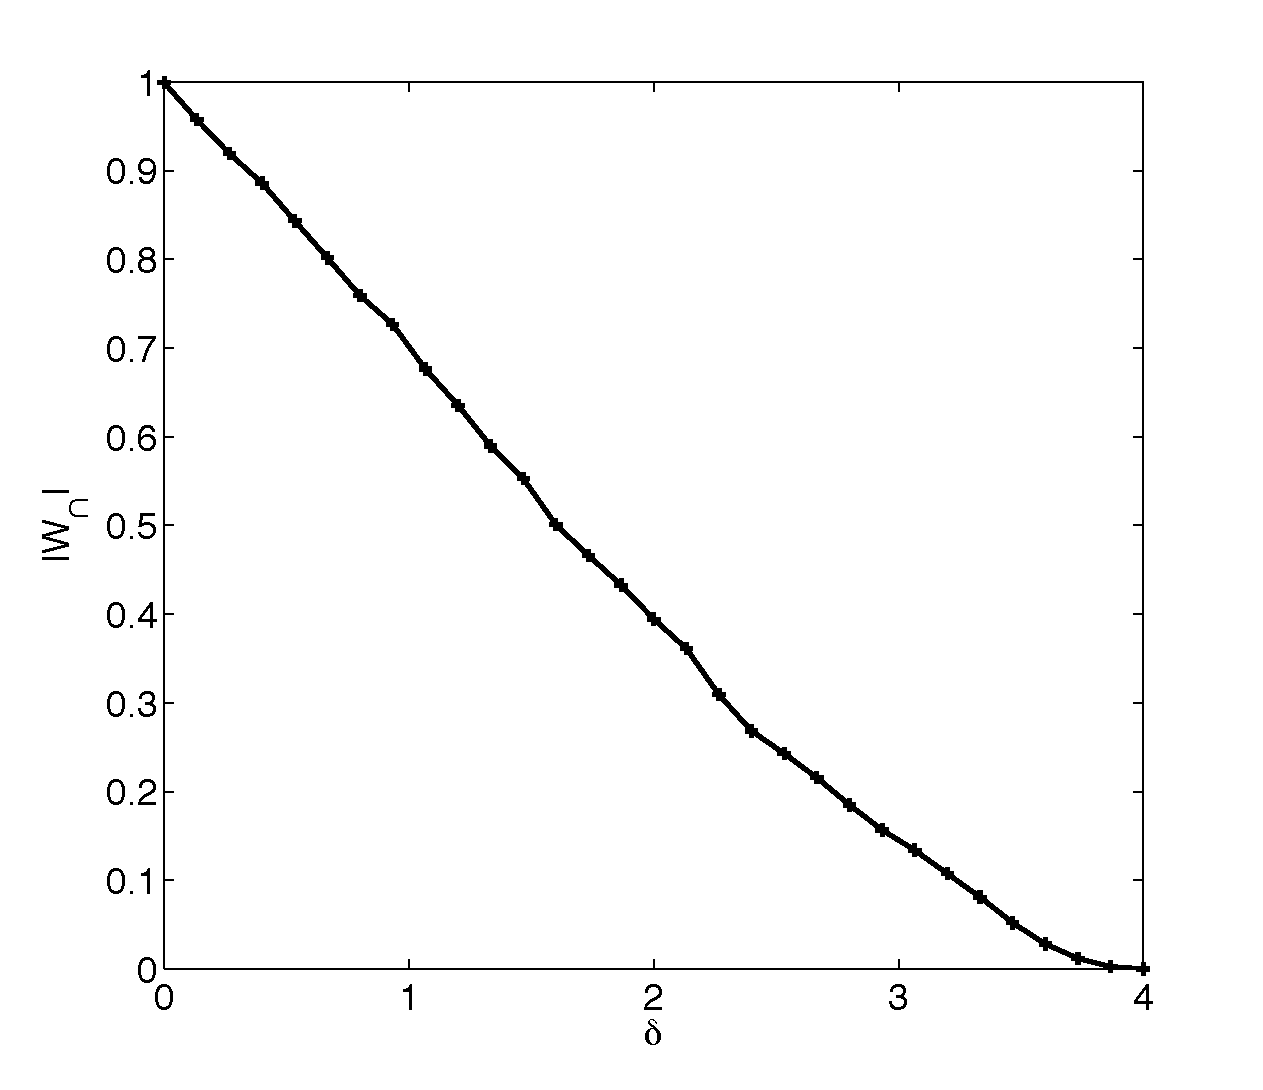
\includegraphics[width=1.5in]{../diagrams/w_capsize.pdf}
\label{fig:w_cap}}
\subfigure[$|W_f|(\delta,\, a)$.]{
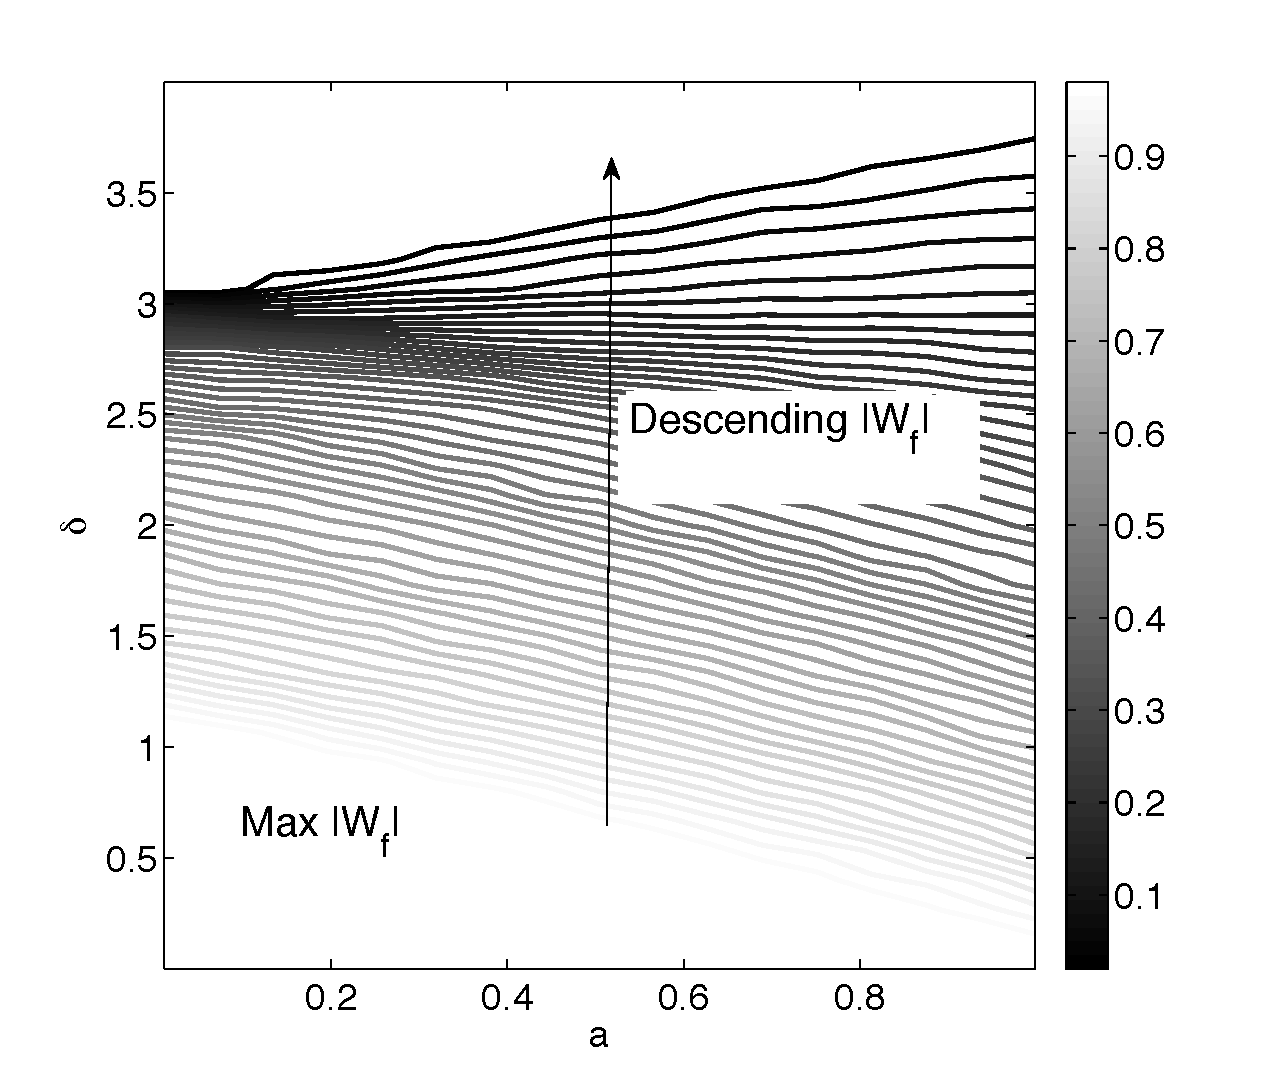
\includegraphics[width=1.5in]{../diagrams/w_fsize.pdf}
\label{fig:w_f}}
\caption{{\small (a): The curve of $|W_\cap|$ in depending on $\delta$ is monotonically decreasing, with some wavering due to low number of points in the sample.  (b):  $|W_f|$ depending on $(\delta,\, a)$.  For small $\delta$,  robot 2 can grasp robot 1 at nearly any point $P$.  As $\delta$ increases, $a$ becomes more important.  For $\delta$ near 4, the distance above which the robots cannot contact each other, there is a small range of $a$ values that give nonempty $W_f$. } }
\end{center}
\end{figure}

The post-failure grasping workspace is more interesting, and depends both on $\delta$ and $a$.  For close placements of robot bases, robot 2 can grasp robot 1 at almost any spot on the second link; $W_f$ is almost identical to $W_1$.  As the robots move further apart,  $\delta$ increases and the region robot 1 can reach while being grasped at $P$ decreases.  Not surprisingly, $|W_f|$ is greatest, for $\delta \in [0 , 2]$ and $a \approx 0$, see Figure~\ref{fig:w_f}.  Thus, we should place a ball joint near the base of joint 2 to ensure largest $W_f$ for closer robot bases.  

As the separation increases so that the workspaces barely overlap, robot 2 may only grasp robot 1 near the end effector, and the resulting $W_f$ is small.    See Figure~\ref{fig:spaceshape}, and column four of  Table~\ref{tab:w_f}.  In these plots, the black area is inaccessible, light gray is fully accessible, and dark gray is reachable from a limited number of configurations.  The inaccessible area clearly increases when $\delta$ is increasing. In general, larger $\delta$ lead to smaller post-failure workspaces for fixed $a$. The converse is not true: $|W_f|$ is not a monotonic function of $a$ for a fixed $\delta$. 
 It is interesting to note that our methods computes explicitly the number of configurations reaching the desired point in a post-failure workspace, even in the case when the configurations belong to isolated domains in the workspace. Such problems are usually challenging for traditional methods of workspace computation. 


Finally, in Figure~\ref{fig:weighted} we show the contour levels of the  objective function $\Omega$ from (\ref{Omegadef}) to determine the optimal ball joint placement.  For weighting factor $\lambda = 0$, $\Omega$ is simply the value of $| W_f |$, and the maximizer for any given $\delta$ is $a = 0$.  With $\lambda  = 1/3$, the optimal joint location is still at the base of the second link, but occurs with separation $\delta = 1$.  Increasing $\lambda$ further makes the size of the intersection workspace overpower the post-failure workspace, and by $\lambda = 2/3$ the maximum of $\Omega$ is invariant with respect to $a$.  Therefore, the weighting factor $\lambda$ plays a critical role in the determination of the optimal grabbing point.

%% Finally, we let the objective function we seek to maximize be $$\Omega = (1-\lambda)\cdot |W_f| + \lambda  (1 - |W_\cap | ). $$  Again, because the two robots are equal, we may normalize the workspace volume to be 1 for each, and let $|W_\cap |$ be the normalized size of the intersection workspace for a given $\delta$ separation distance. 
\vskip0.2cm
\begin{figure}[t]
\begin{center}
\subfigure[$\lambda = 0$.]{
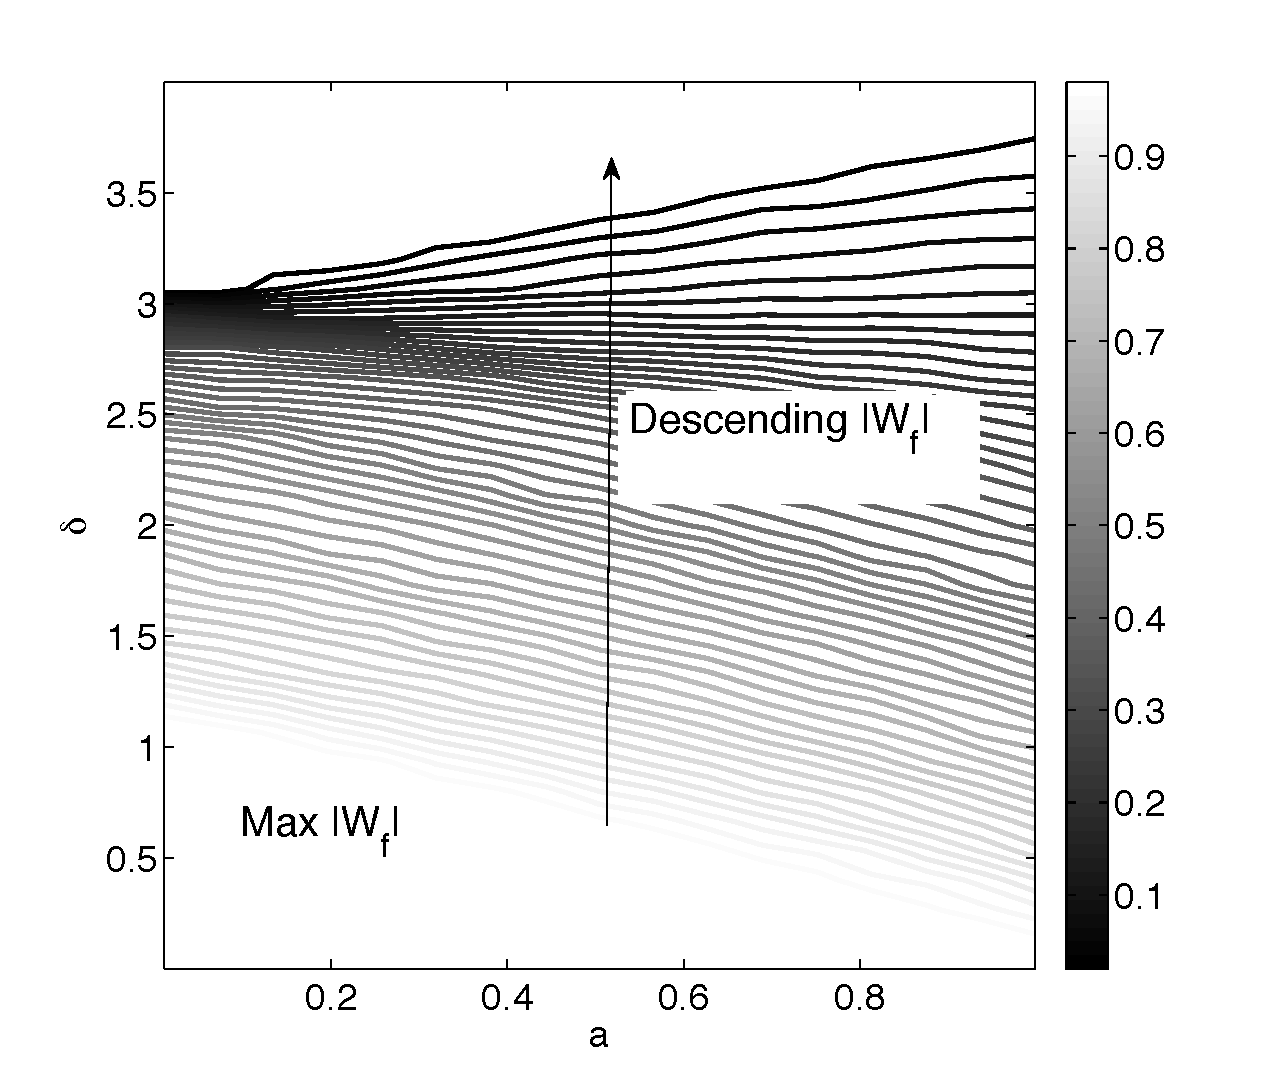
\includegraphics[width=1.5in]{../diagrams/w_fsize.pdf}
\label{fig:weighted_0}}
\subfigure[$\lambda = 0.333$.]{
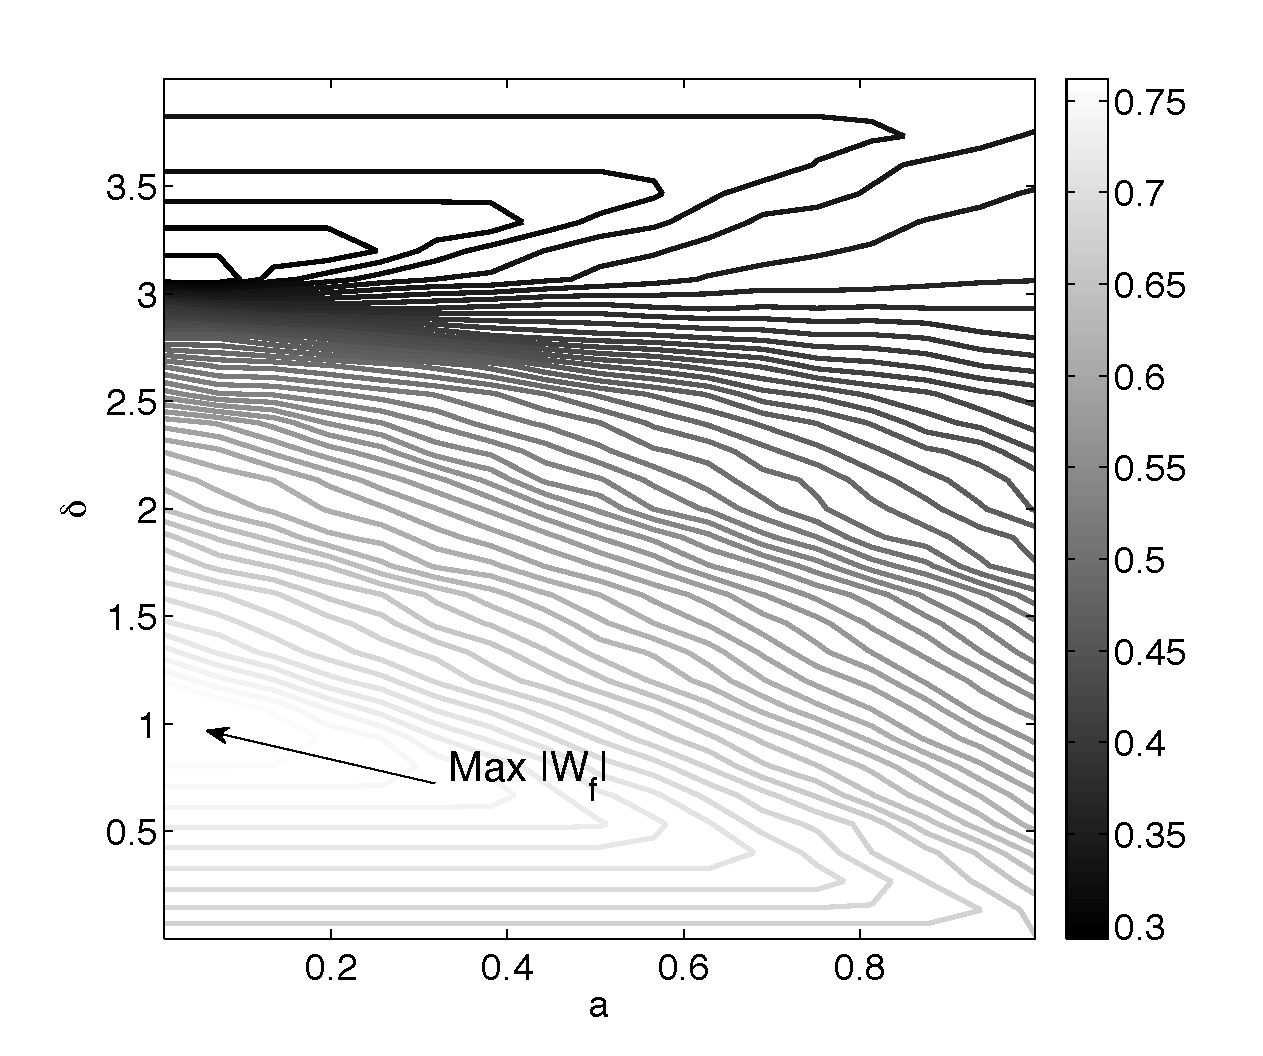
\includegraphics[width=1.5in]{../diagrams/weighedsum_0333.pdf}
\label{fig:weighted_0333}}

\subfigure[$\lambda = 0.666$.]{
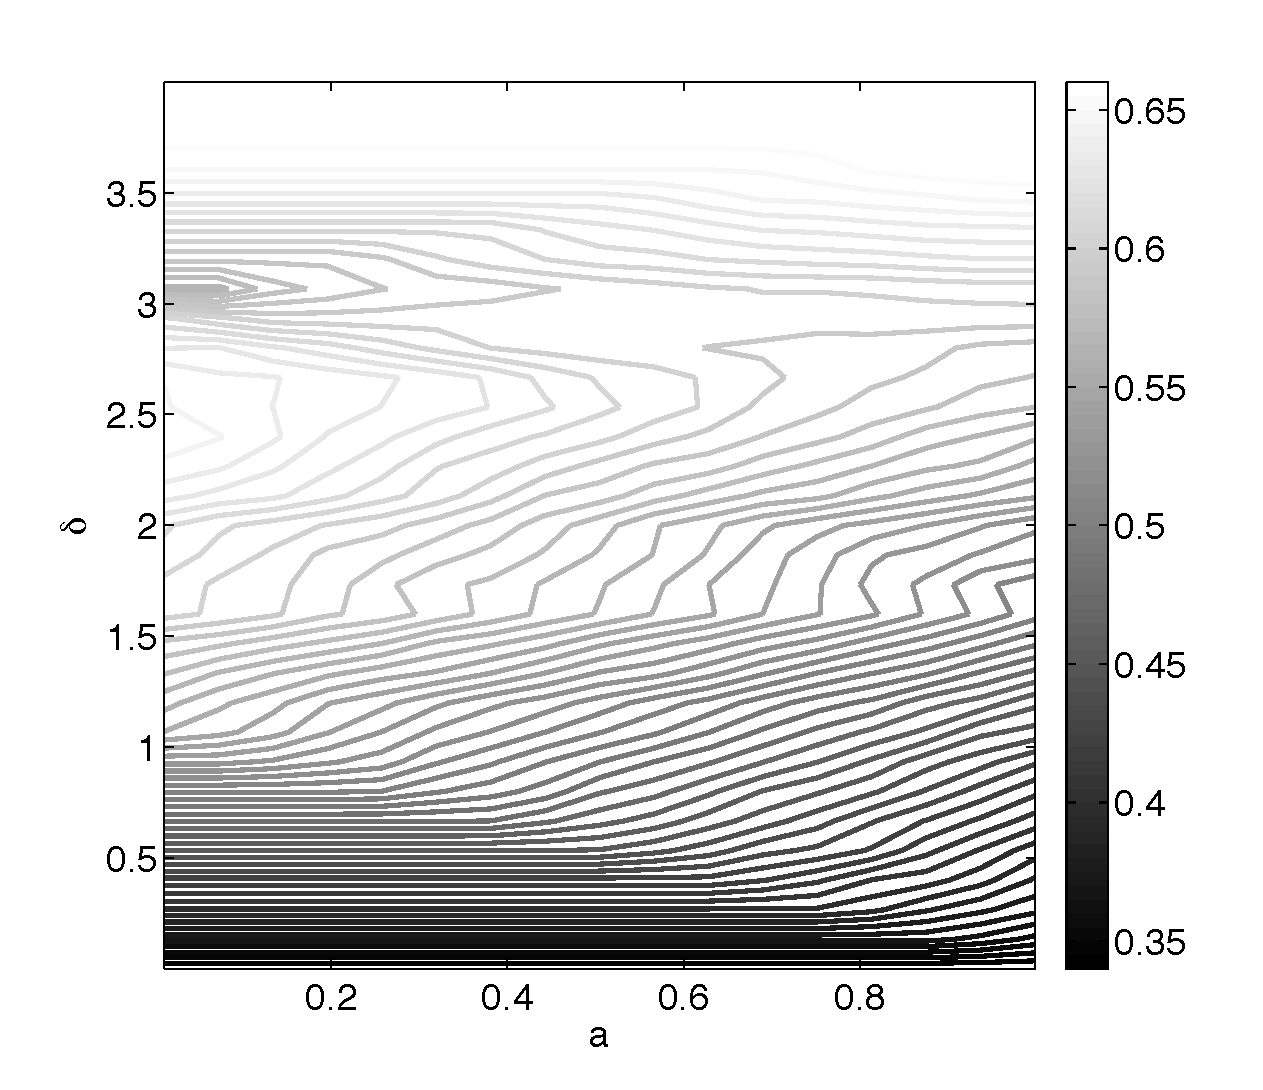
\includegraphics[width=1.5in]{../diagrams/weighedsum_0666.pdf}
\label{fig:weighted_0666}}
\subfigure[$\lambda = 1$.]{
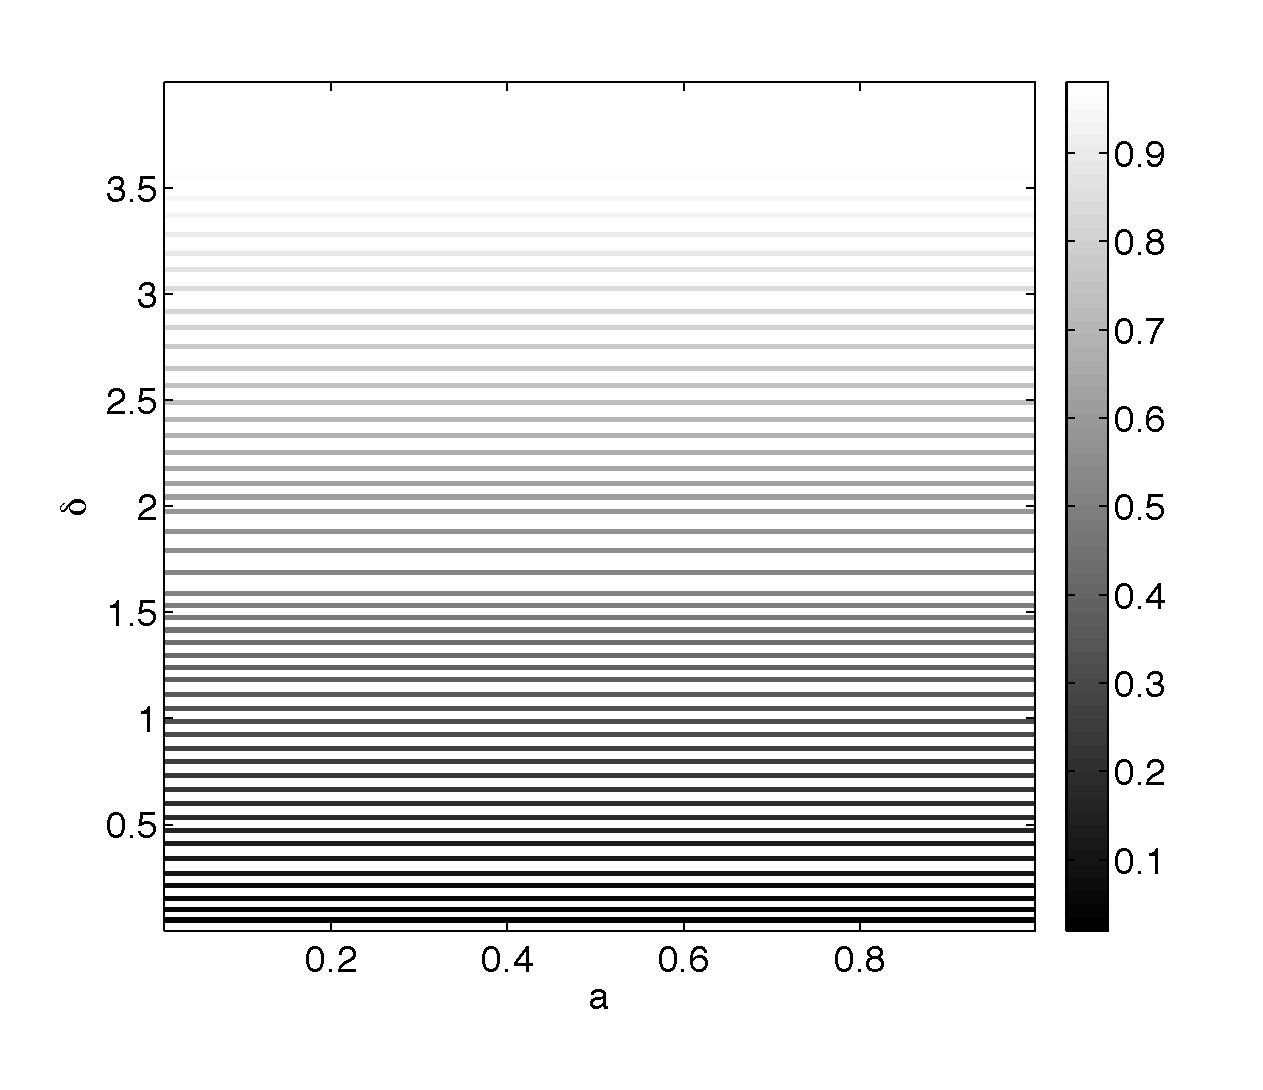
\includegraphics[width=1.5in]{../diagrams/weighedsum_1.pdf}
\label{fig:weighted_1}}

\caption{\small Objective function contours for a grid of $(\delta , \, a)$ pairs for 2D cooperating robots.  }
\label{fig:weighted}
\end{center}
\end{figure}


\section{3D Case: Three Joint Manipulators} \label{sec:threejoint}

Equations determining the kinematics of three dimensional robots are more complicated than those of planar manipulators. This concerns both the higher number of relevant equations, due to the higher number of links in a typical 3D robots, and the structure of equations describing the motions. Yet, the method for optimizing cooperative workspaces remains fundamentally the same, as those equations can be brought to an algebraic form and then solved using the methods outlined above in Section~\ref{sec:workspacecomputation}. Thus for the sake of brevity, in this section we only write a sketch of the method in 3D. 
% because there are three links for the failed robot, we compute three distinct post-failure workspaces as one per link.  

In the example for this section, we consider two cooperating PUMA robots, ignoring orientation of the end effector.   There is some disagreement in the relevant literature regarding which parameters should be used in describing such a robot \cite{consensus} . In this paper, we use DH parameters defined as in Table~\ref{tab:pumadh}. Treating the first three links of the PUMA as our robot, we ignore the wrist; we do this to limit the curse of dimensionality and reduce the number of points to analyze.  Instead, we use a tool frame to translate from the arm to the end effector.  The frame we used retains the orientation of the arm, and translates along the final $z$-axis by 0.4331 meters.


\vskip0.3cm
\begin{table}
\begin{center}
\caption{Denavit-Hartenberg Parameters for PUMA robot.}
\label{tab:pumadh}
\begin{tabular}{| c | c | c | c | c | c |}
\hline
$\theta_i$			&	$\alpha_i$			&	$a_i$ (m)	&	$d_i$ (m)		&  $\theta_{i,min}$	&	$\theta_{i,max}$\\ \hline
$\theta_1$ 		&	0					& 	0		&	0			& $-160^\circ$	& $160^\circ$ \\
$\theta_2$ 		&	$-\pi/2$				& 	0.4318		&	0.2435		&$-225^\circ$	& $45^\circ$	\\
$\theta_3$		&	0					&	$-0.0203$		&	$-0.0934$		&$-45^\circ$	& $225^\circ$	\\
$\theta_4$		&	$\pi/2$				&	0		&	0.4331		&$-110^\circ$	& $170^\circ$	\\
$\theta_5$		&	$-\pi/2$				&	0		&	0			&$-100^\circ$	& $100^\circ$	\\
$\theta_6$		&	$\pi/2$				&	0		& 	0.5625			&$-266^\circ$	& $266^\circ$	 \\ 
\hline
\end{tabular}
\end{center}
\end{table}


In order to save space and simplify the computations, we shall only consider the robots cooperating through the first three links.  Also, we assume the bases to be coplanar, and the robots to be oriented with respect to this plane in the same direction; this allows us to parametrize the separation of the PUMAs with only one parameter.  Each of the workspaces $W_1$, $W_2$, $W_\cap$ will have six equations in six variables, which are solved via \bertini \, after bringing the trigonometric part of these equations into algebraic form.  Correspondingly,  there will be  12 equations defining the  post-failure workspaces with 12  variables; these equations appear in Appendix \ref{app:eqns}.  
The space of possible positions for each manipulator is now a subset of $\R^3$. In order to find $W_{1,2}$ we sample randomly an oversized rectangular box surrounding the robot, which will include the workspace. In order to determine good bounds for the workspaces, we first do forward kinematics by randomly sampling the three joint variables $\theta_i \in [0,2 \pi]$. The result of this estimate is that the cubic box  $[ -0.9,\, 0.9 ] \times [ -0.9,\, 0.9 ] \times [ -0.9,\, 0.9]$ contains $W_i$, and is thus a good starting point for finding the cooperative workspaces in which we are interested. 



The PUMA has joint limits that reduce its workspaces significantly. The limits we use for this example appear in Table~\ref{tab:pumadh}.  because joint limits are written as inequalities $\theta_{i,min} \leq \theta_i \leq \theta_{i,max}$, they are not algebraic equations.     There are two possibilities for dealing with this problem. One could compute the workspace boundaries at the joint limits $\theta_i=\theta_{i,max}$ and $\theta_i=\theta_{i,min}$. However, these constraints do not always lead to meaningful boundaries in cooperating workspaces, and even when they do, it is often hard to define the volumes they bound. Instead, we simply use these joint limits in post-processing, only selecting the suitable  joint angles among all real solutions.  

\begin{figure}
\begin{center}

\subfigure{
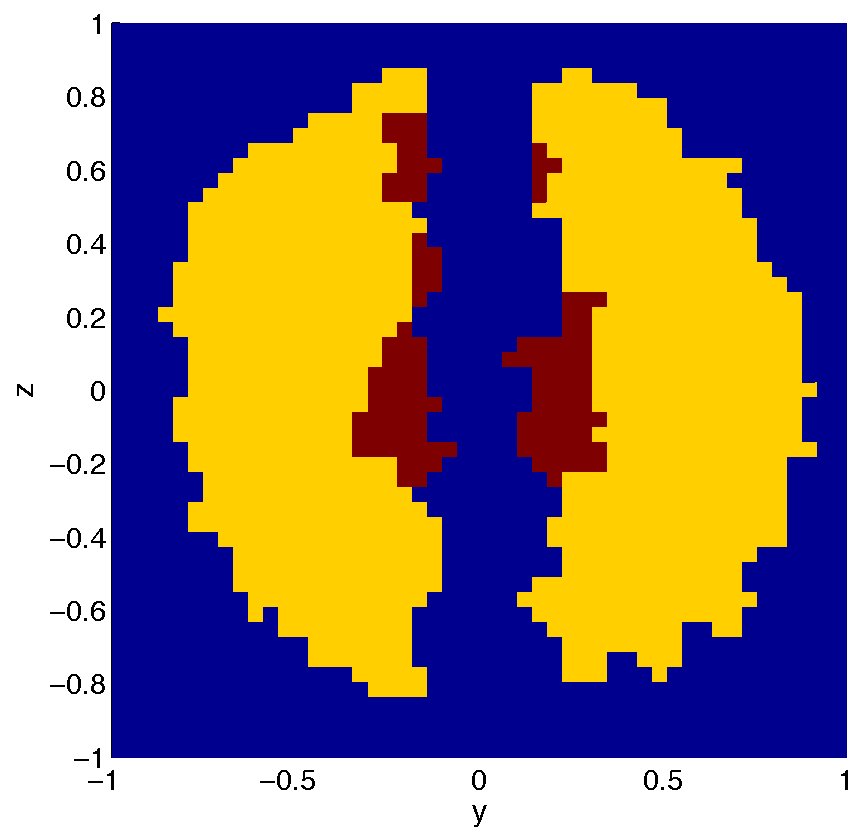
\includegraphics[width=1.5in]{../diagrams/xslice_limit.pdf}}
\subfigure{
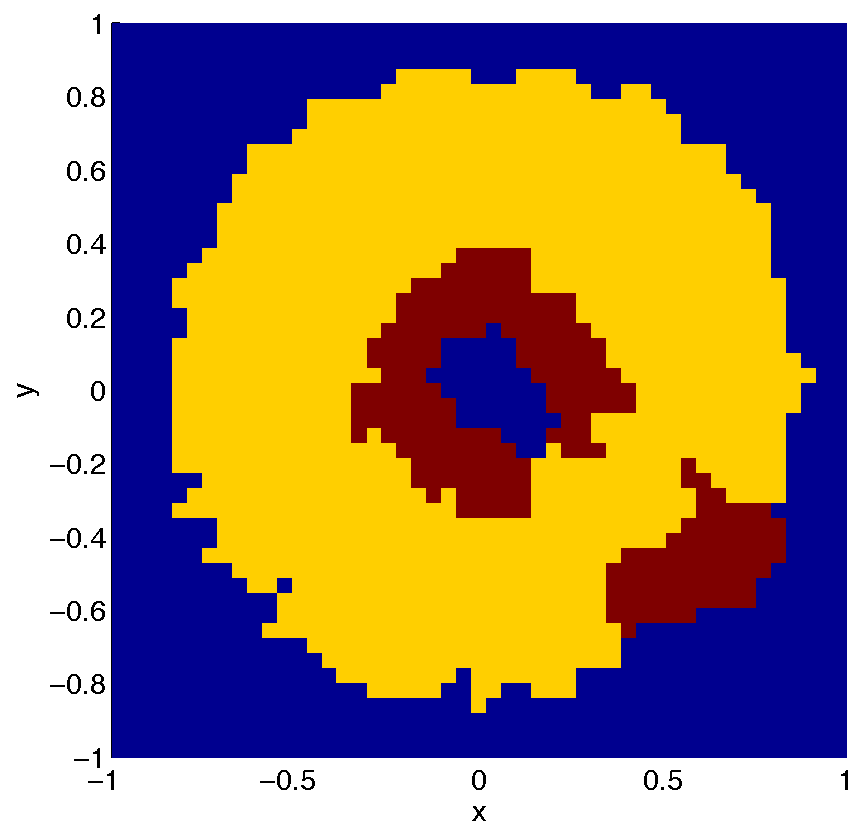
\includegraphics[width=1.5in]{../diagrams/zslice_limit.pdf}}

\subfigure{
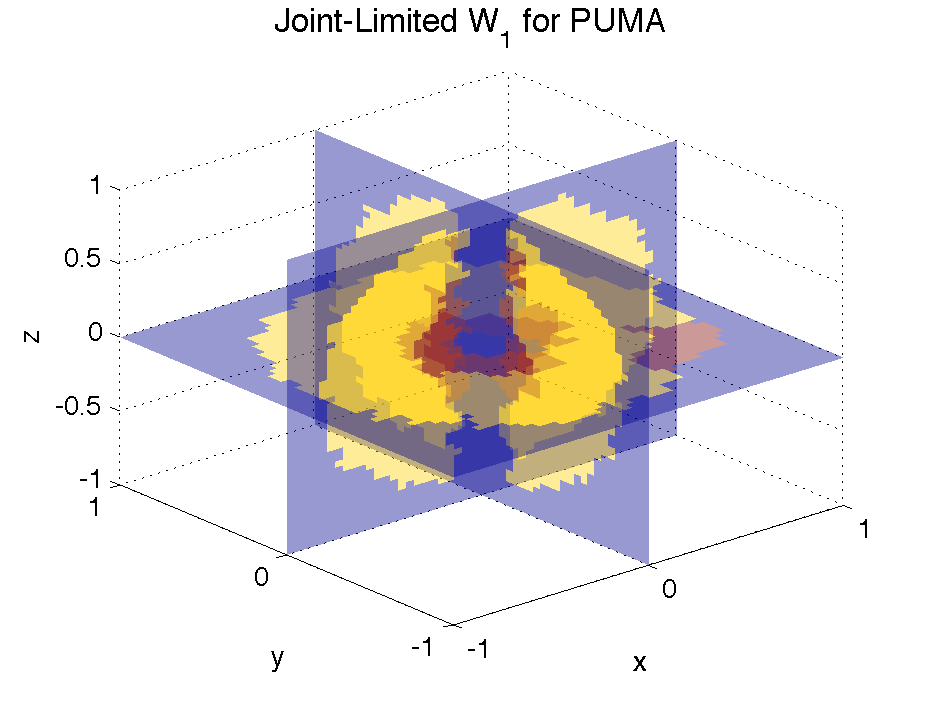
\includegraphics[width=3.05in]{../diagrams/puma_init_limited.pdf}}

\caption{
Top: Slices of the pre-failure PUMA workspace $W_1$ by the planes $x=0$ (left) and $z=0$ (right). Bottom: Combined picture of workspace with three slices $x=0$, $y=0$, $z=0$. Yellow color: areas accessible the angles satisfying joint limits  given in Table~\ref{tab:pumadh}. Red color: real solutions violating joint limits. Dark blue region: inaccessible. 
}
\label{fig:3dworkspaces}
\end{center}
\end{figure}

%\comment{almost there: include a graphic for pre-failure , intersection, and post-failure workspaces.}
Our results for  various workspaces are shown  in Figure~(\ref{fig:3dworkspaces}).  These data are based on 10,000 points in the $(x,y,z)$ space.  Of particular interest here is  the presence of  voids inside of all  workspaces.   Because the data plotted is generated from a random sampling, to plot nicely we called the Matlab method \texttt{griddata}, and the result is a blocky pseudo-color plot.  Forbidden area is represented by the dark blue color. The red and yellow colors show the accessible work space, with the yellow areas being accessible only if the joint limits are satisfied. The resulting workspace is essentially a torus, although the particular realization we have chosen makes it hard to visualize this as a volume in the 3D space, because of the relative narrowness of the ``hole". Instead, we have chosen to represent the workspace through the slices. Two slices by the planes $x=0$ and $z=0$ are shown in the top of the Figure, and the combined figure presenting the slices is shown in the bottom. The voids in $W_i$ come from the offsets of the arm, and they expand  for cooperating robots. Our results show that great care needs to be taken in designing and arranging robotic arms for cooperation, as it may lead to large inaccessible regions of  workspace. 


\begin{figure}
\begin{center}
\subfigure[ $|W_\cap|$ vs $\delta$.]{
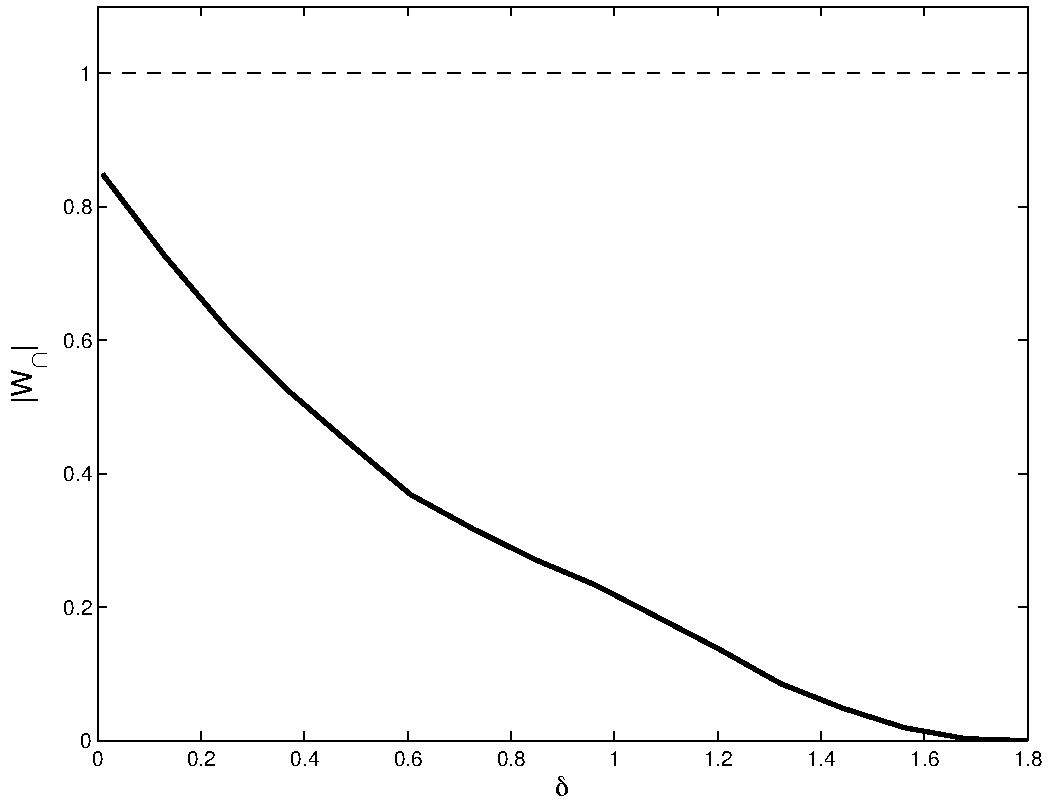
\includegraphics[width=1.5in]{../diagrams/epsnonisect1.pdf}}
\subfigure[$\lambda=0$.]{
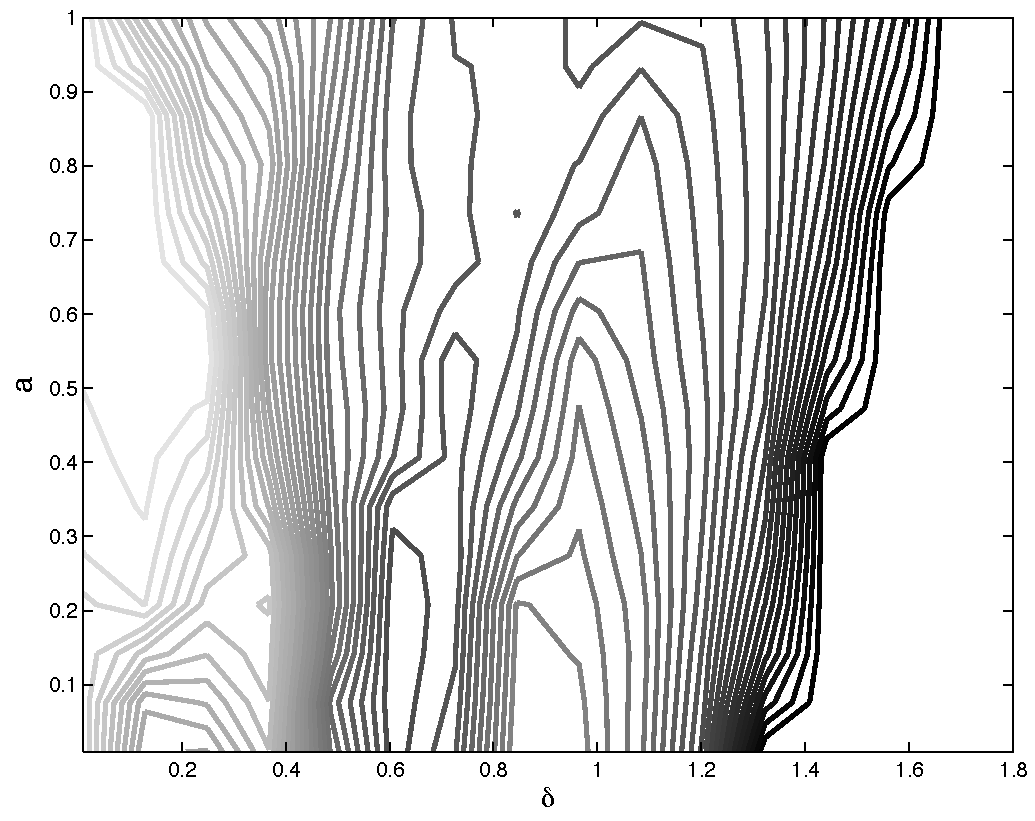
\includegraphics[width=1.5in]{../diagrams/epsomega_contour1_0link2.pdf}}

\subfigure[$\lambda = 1/3$.]{
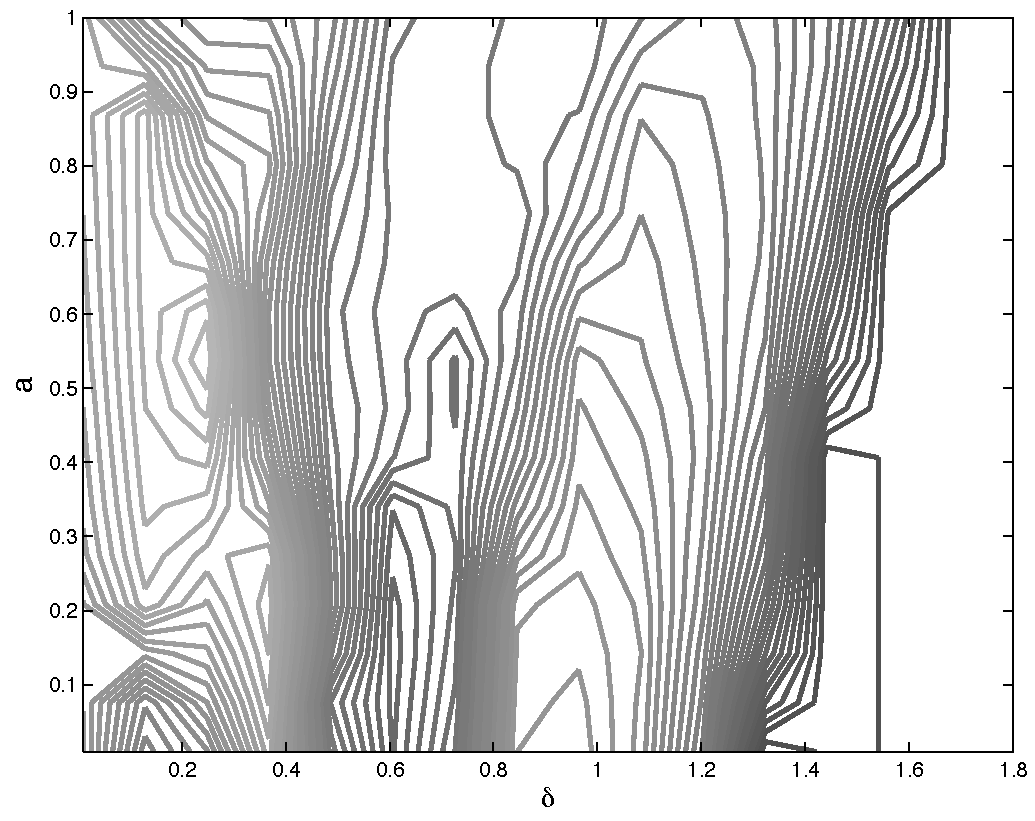
\includegraphics[width=1.5in]{../diagrams/epsomega_contour1_033333link2.pdf}}
\subfigure[$\lambda = 2/3$.]{
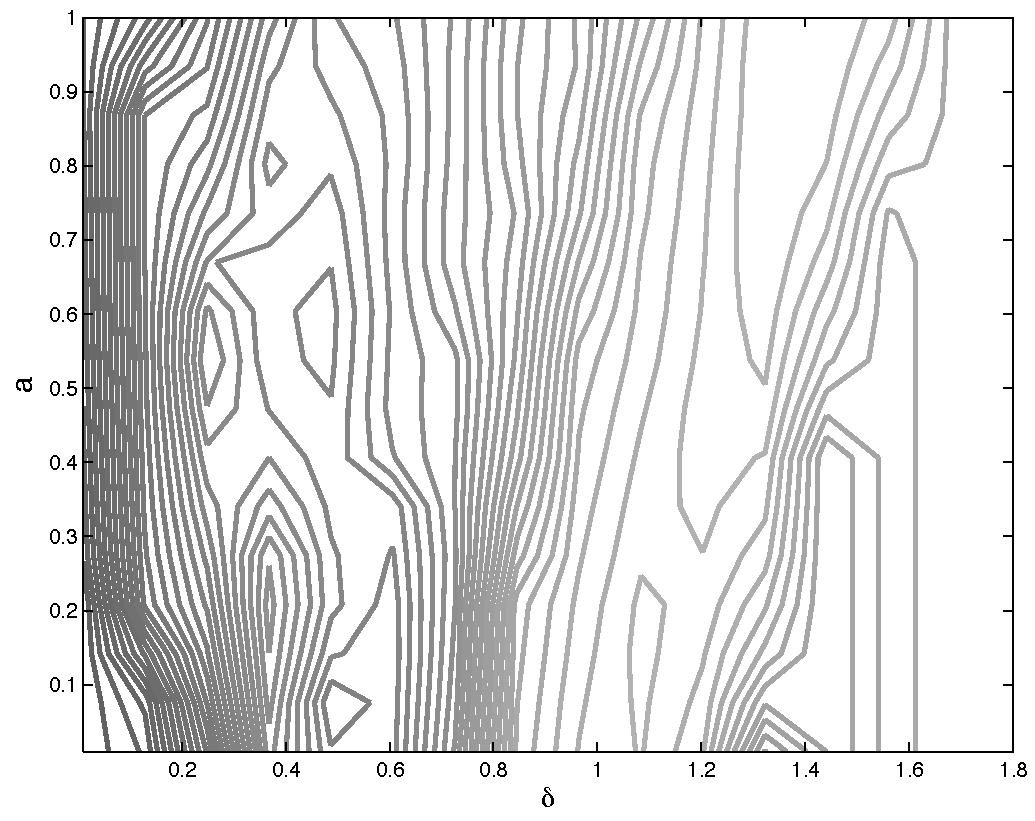
\includegraphics[width=1.5in]{../diagrams/epsomega_contour1_066667link2.pdf}}

\label{fig:objective3d}
\caption{Considering grasping on the second link to restore workspace after failure of joint 2 of a PUMA robot.  a) Measurement of the intersection workspace $|W_\cap|$, as a function of $\delta$. 
 b)-d) Contours of the objective function $\Omega$ versus $(\delta,a)$ for 3D cooperating robots. Note that for the case b), $\lambda=0$ and the objective function $\Omega$ is equal to the measure of post-failure workspace $|W_f|$. 
 }
\end{center}
\end{figure}





We also present the plot of objective function versus parameters $\delta$ and $a$ in Figure~\ref{fig:objective3d}, chosen to extend the  results presented above for 2D robots.  To calculate  $\Omega$, we compute each of the workspaces $W_1$, $W_\cap$ and $W_f$.  Initially, $W_1$ is determined using the results shown in Figure~\ref{fig:3dworkspaces}, computed with $10^4$ points.  Then $W_\cap$ is computed over a discretization of $0 \leq \delta \leq 1.8$ into 16 values.  Finally, we compute $W_f$, for a particular value of $\delta$ and $a$. The results are repeated over a $16 \times 16$ regular grid of $0\leq \delta \leq 1.8$, and $0\leq a \leq 1$, and considering grasping the failed robot on each of the three possible links. Thus, the total number of parameter combinations we considered for $W_f$ is $7.68 \cdot 10^6$. However, we do not need to treat that many paths by \bertini, as we throw out the space samples that are not in the initial workspace for subsequent computations.


The objective function landscapes presented in Figure~\ref{fig:objective3d} for the PUMA robot are very similar to those for the 2D planar robot above in Figure~\ref{fig:weighted}.  Because each joint could fail independently of the others, we need to consider a grasping location for each link of the robot; hence, we have an objective function landscape for each of the three links of the PUMA.  However, the landscapes are similar, so only those for the second link are presented here. The values of $|W_\cap|$ monotonically decrease with increase of $\delta$, with $W_1 = W_\cap$ for $\delta = 0$.  For results on $W_f$, we average over the sizes of $W_f$ for grasping on each link, at normalized distance $a$ from the base.  This would be user-defined in practice; for example, if we knew the third joint was most likely to fail, we might compute $\Omega$ using only $W_f$ for this joint.  This extra information will also give substantial computational savings. 

	As with the 2D example above, the weighting factor $\lambda$ plays a crucial role in optimizing.  The limiting cases of $\lambda=1$ and $\lambda=0$ return simply $(1 - |W_\cap|)$ or $|W_f|$ respectively.  Around $\lambda = 2/3$, we are more concerned with maximizing pre-failure workspace.  The maximum values of $\Omega$ appear at the right of the figure, with large separation between the robots.  Around $\lambda = 1/3$, we put more emphasis on increasing the remainder of workspace accessible in grasping configuration;. For that value of $\lambda$, objective function  $\Omega$ is mostly flat, with a rise near $\delta = 0.2$, and $a = 0.5$.  The optimal distance and grasping location depends on the link, and on the weighting factor, making user preference crucial in the optimization procedure. 


\section{Conclusion}


We used homotopy continuation, as implemented in \emph{Bertini}, to estimate the size of workspaces, the intersection of workspaces, and post-failure grasping workspaces in the case of having two  serial robots placed near one another, in two and three dimensions. We also solve the problem of the optimal configuration for these robots for one example of a user-defined objective function.  A general algorithm for solving the problem of finding optimal placement and configuration of two such robots was also presented.   

Yet again, one could get some results for this optimization problem using standard methods, such as Jacobian control.  However, by using algebraic geometric methods, we avoid issues such as isolated domains and multiple solutions to inverse kinematics equations.  For example, multiple isolated solutions can appear even in the pre-failure workspace in the case of a robot having to work around an obstacle, with the target reachable in multiple ways. The homotopy continuation algorithms will not encounter any difficulty in that case, whereas the Jacobian control method will need to be augmented with the specific knowledge from the problem and yet fail to find all isolated solutions. Our algorithm can be extended to more general cases.  For example,  it will be relatively straightforward to  account for different designs for the two robots (including unequal link lengths) or introduce the dynamical load variables in the objective function.  Also, methodological choices in the algorithm, such as the use of homotopy continuation, have been made to make the 
generalization  to higher-dimensional workspaces possible. 

It should be noted that the methods of numerical algebraic geometry may be used to compute {\em complex} positive-dimensional components of the solutions sets of polynomial systems.  However, it is nearly impossible to detect positive-dimensional {\em real} solutions, particularly above dimension one.   Therefore, kinematically redundant robots present difficulty for our method.  Perhaps we could systematically reduce the underconstrained inverse kinematic system for such a robot to a fully constrained system; however, the curse of dimensionality will likely be problematic.  This is a direction of ongoing research.

One can say even though the method is highly comprehensive,  the disadvantage lies in the relative computation intensity and large number of data generated by the method. 
In particular, all the results in this paper have been obtained on a 72-core Dell cluster; the PUMA data took about 24 hours to generate. We shall note we tried to keep the algorithm as general as possible, without referring to the knowledge of particular workspace or robotic geometries, that may speed up the computation considerably. Also,  because the homotopy continuation algorithm is pleasantly parallel, for practical applications it can be extended to run with high efficiency on modern GPU workstations. Thus, even though the computations for this paper took considerable time, it is not inconceivable that it can be made to run for real-time robot guidance in the near future. 




% if have a single appendix:
%\appendix[Proof of the Zonklar Equations]
% or
%\appendix  % for no appendix heading
% do not use \section anymore after \appendix, only \section*
% is possibly needed

% use appendices with more than one appendix
% then use \section to start each appendix
% you must declare a \section before using any
% \subsection or using \label (\appendices by itself
% starts a section numbered zero.)
%

\newpage
\section{eqns}

\label{app:eqns}
The inverse kinematic equations for the first three joints of the PUMA robot are, as used in this paper are $f_i=0$ for $i=1,\ldots,12$ with $f_i$ defined as:
\begin{align*}
f_1 =& 0.4318 c_1 c_2 - 0.2435 s_1 + 0.0934 a s_1 + 0.4331 c_1 c_2 s_3 + \\
	&0.4331 c_1 c_3 s_2 + 0.0203 a c_1 s_2 s_3 - 0.0203 a c_1 c_2 c_3 - \\
	&(0.4318 c_4 c_5 - 0.1501 s_4 - 0.0203 c_4 c_5 c_6 + \\
	&0.4331 c_4 c_5 s_6 + 0.4331 c_4 c_6 s_5 + 0.0203 c_4 s_5 s_6+\delta)\\
f_2 =& 0.2435 c_1 - 0.0934 a c_1 + 0.4318 c_2 s_1 + 0.4331 c_2 s_1 s_3 + \\
	&0.4331 c_3 s_1 s_2 + 0.0203 a s_1 s_2 s_3 - 0.0203 a c_2 c_3 s_1 - \\
	&(0.1501 c_4 + 0.4318 c_5 s_4 - 0.0203 c_5 c_6 s_4 + \\
	&0.4331 c_5 s_4 s_6 + 0.4331 c_6 s_4 s_5 + 0.0203 s_4 s_5 s_6)\\
f_3 =& 0.4331 c_2 c_3 - 0.4318 s_2 - 0.4331 s_2 s_3 + 0.0203 a c_2 s_3 + \\
	&0.0203 a c_3 s_2 - (0.4331 c_5 c_6 - 0.4318 s_5 + 0.0203 c_5 s_6 + \\
	&0.0203 c_6 s_5 - 0.4331 s_5 s_6)\\
f_4 =& 0.4318 c_1 c_2 - 0.1501 s_1 - 0.0203 c_1 c_2 c_3 + \\
	&0.4331 c_1 c_2 s_3 + 0.4331 c_1 c_3 s_2 + 0.0203 c_1 s_2 s_3 - x\\
f_5 =& 0.1501 c_1 + 0.4318 c_2 s_1 - 0.0203 c_2 c_3 s_1 + \\
	&0.4331 c_2 s_1 s_3 + 0.4331 c_3 s_1 s_2 + 0.0203 s_1 s_2 s_3 - y\\
f_6 =& 0.4331 c_2 c_3 - 0.4318 s_2 + 0.0203 c_2 s_3 + \\
	&0.0203 c_3 s_2 - 0.4331 s_2 s_3 - z\\
f_7 =& s_1^2+c_1^2-1\\
f_8 =& s_2^2+c_2^2-1\\
f_9 =& s_3^2+c_3^2-1\\
f_{10} =& s_4^2+c_4^2-1\\
f_{11} =& s_5^2+c_5^2-1\\
f_{12} =& s_6^2+c_6^2-1
\end{align*}

The coefficients appearing in these equations are 4 digit approximations of exact numbers coming from the DH parameters for the PUMA.  The terms $x, y, z, \delta, a$ appear in the equations as parameters for \bertini.  Functions $f_1 - f_6$ couple the positions of the two cooperating robots, and functions $f_7 - f_{12}$ are Pythagorean identities tying cosines and sines together.



\chapter{Conclusion}

\bibliographystyle{plain}
\bibliography{brakedissertation}
%\printindex





\end{document}  
